\documentclass[12pt,a4paper]{article}
\usepackage[utf8]{inputenc}
\usepackage[T1]{fontenc}
\usepackage{geometry}
\usepackage{graphicx}
\usepackage{amsmath}
\usepackage{amsfonts}
\usepackage{amssymb}
\usepackage{booktabs}
\usepackage{longtable}
\usepackage{array}
\usepackage{multirow}
\usepackage{wrapfig}
\usepackage{float}
\usepackage{colortbl}
\usepackage{pdflscape}
\usepackage{tabu}
\usepackage{threeparttable}
\usepackage{threeparttablex}
\usepackage{forloop}
\usepackage{calc}
\usepackage{hyperref}
\usepackage{url}
% \usepackage{cite}
\usepackage{natbib}
\usepackage{setspace}
\usepackage{fancyhdr}
\usepackage{lastpage}
\usepackage{titlesec}
\usepackage{tocloft}
\usepackage{enumitem}
\usepackage{xcolor}
\usepackage{listings}
\usepackage{inconsolata}

% Page setup
\geometry{margin=1in}
\setlength{\parindent}{0pt}
\setlength{\parskip}{6pt}
\setlength{\headheight}{15pt}

% Header and footer
\pagestyle{fancy}
\fancyhf{}
\rhead{Income Inequality and Poverty Dynamics}
\lhead{Statistical Analysis Report}
\rfoot{Page \thepage\ of \pageref{LastPage}}

% Title formatting
\titleformat{\section}{\Large\bfseries}{\thesection}{1em}{}
\titleformat{\subsection}{\large\bfseries}{\thesubsection}{1em}{}
\titleformat{\subsubsection}{\normalsize\bfseries}{\thesubsubsection}{1em}{}

% Code listing setup
\lstset{
    basicstyle=\ttfamily\small,
    breaklines=true,
    frame=single,
    numbers=left,
    numberstyle=\tiny,
    showstringspaces=false,
    tabsize=2
}

% Hyperref setup
\hypersetup{
    colorlinks=true,
    linkcolor=blue,
    filecolor=magenta,      
    urlcolor=cyan,
    citecolor=red
}

\begin{document}

% Title information
\title{Income Inequality and Poverty Dynamics - A Global Analysis of Economic Development Patterns}
\author{Basir Abdul Samad \\
Statistical Computing Project Report \\
Baruch College, Weissman School of Arts and Sciences}
\date{\today}

\maketitle

\begin{abstract}
Our study examines how income distribution affects poverty reduction across countries from 1970 to 2024. Using six complementary datasets, we find compelling evidence that inequality significantly moderates the effectiveness of economic growth in reducing poverty. Our most comprehensive regression model explains 57.9\% of variance in poverty rates and reveals a significant interaction effect (-0.983, p < 0.001) between income and inequality. This translates to dramatic real-world consequences: a 10\% increase in mean income reduces poverty by 0.78 percentage points in countries with moderate inequality (richest-to-poorest ratio of 5), but only by 0.29 percentage points in highly unequal countries (ratio of 10). These findings are reinforced by our success case analyses: countries like Malaysia, Chile, and Costa Rica, which combined economic growth with stable or decreasing inequality, achieved over 96\% reduction in extreme poverty. Regional comparisons further support this pattern, with East Asia experiencing the most dramatic poverty reduction while maintaining moderate inequality levels, unlike more unequal regions like Latin America. Our findings demonstrate that development strategies must address both economic growth and distributional patterns to effectively combat poverty.
\end{abstract}

\tableofcontents
\listoffigures
\newpage

\section{Introduction}\label{sec:introduction}
Global poverty reduction remains one of the most pressing challenges of our time. While significant progress has been made in reducing extreme poverty over recent decades, the benefits of economic growth have not been distributed equally across and within countries. Traditional approaches to measuring economic development have often focused on aggregate metrics like GDP growth or mean income, which can mask important distributional patterns.

Our ultimate goal in this project was to determine whether and how income inequality affects poverty reduction efforts. Specifically, we sought to discover if countries with lower income inequality experience greater poverty reduction for a given level of economic growth. This question has profound implications for development policy, if inequality impedes poverty reduction, then strategies focusing solely on economic growth might be insufficient.

Understanding how economic prosperity is shared across different segments of society, particularly how economic growth affects the poorest populations, requires more nuanced analysis that considers both income levels and income distribution. The central question driving our research is: How does income distribution affect the relationship between economic growth and poverty reduction?

We achieved our goal through a comprehensive analysis of six complementary datasets from Our World in Data \cite{hasell2022poverty}, covering various aspects of income distribution and poverty across countries from 1970 to 2024. By calculating inequality metrics like the mean-to-median ratio and richest-to-poorest decile ratio, we were able to quantify income distribution patterns. Through correlation analysis, regression modeling, and time series decomposition, we established the relationships between these inequality measures and poverty reduction rates. Our regional and country-specific analyses further revealed how these relationships vary across different contexts.

The specific objectives of our study were:
\begin{enumerate}
    \item Analyze how income distribution shapes the relationship between economic growth and poverty reduction
    \item Compare different measures of inequality and their correlation with poverty reduction rates
    \item Identify countries that have successfully reduced both poverty and inequality
    \item Investigate how growth rates of different income segments relate to overall poverty reduction
    \item Develop models that predict poverty reduction based on growth patterns and income distribution
\end{enumerate}

As our analysis will demonstrate, we achieved these objectives and found compelling evidence that inequality does indeed affect poverty reduction, specifically, our regression models showed that economic growth is more effective at reducing poverty in more equal societies, confirming our initial hypothesis and providing valuable insights for development policy.

\section{Data Collection and Description}\label{sec:data}
Our analysis integrates six complementary datasets that together provide a comprehensive view of global income distribution and poverty dynamics:
\begin{enumerate}
    \item \textbf{Mean Income or Consumption Per Day:} Contains average daily income/consumption values for countries from 1970-2024. The dataset includes 2,705 country-year observations with values ranging from \$0.997 to \$93.328 per day.
    \item \textbf{Median Income or Consumption Per Day:} Contains the middlemost value of income distribution (50th percentile) for the same countries and time periods. Values range from \$0.690 to \$79.700 per day across 2,705 observations.
    \item \textbf{Poorest Decile Threshold:} Contains the income threshold marking the poorest 10\% of the population by country and year. Values range from \$0.250 to \$37.034 per day.
    \item \textbf{Richest Decile Threshold:} Contains the income threshold marking the richest 10\% of the population. Values range from \$1.578 to \$167.603 per day.
    \item \textbf{Number of People Below Poverty Lines:} Contains absolute numbers of people living below eight different poverty thresholds (\$1, \$2.15, \$3.65, \$6.85, \$10, \$20, \$30, and \$40 per day) across 2,705 observations.
    \item \textbf{Share of Population Below Poverty Lines:} Contains the percentage of each country's population living below the same eight poverty thresholds across 1,468 observations.
\end{enumerate}

Initial data exploration revealed minimal missing values in the income distribution datasets (approximately 70-72 missing values out of 2,705 observations, representing just 2.6\% of the data), while the poverty datasets contained no missing values. The datasets cover a wide range of countries, including developed economies like the United States and Germany, rapidly growing economies like China and India, and developing regions in Latin America and Sub-Saharan Africa.

The datasets were obtained from publicly available sources \cite{hasell2022poverty} and represent standardized measures of income and poverty, allowing for cross-country comparisons. All monetary values are expressed in international dollars adjusted for purchasing power parity (PPP), enabling meaningful comparisons across countries and time periods.

\section{Methodology}\label{sec:methodology}
Our analysis employed several statistical and data visualization techniques implemented in R:
\begin{enumerate}
    \item \textbf{Data Integration:} We merged the six datasets to create a comprehensive analytical framework that allows for examining relationships between income distribution metrics and poverty measures. The integration resulted in a dataset containing 1,462 country-year observations with complete data across all variables.
    \item \textbf{Inequality Metrics Calculation:} We calculated three primary inequality metrics to compare income distribution patterns across countries: 
    \begin{itemize}
        \item \textbf{Mean-to-median ratio} = Mean Income / Median Income. This ratio measures the skewness of income distribution. A ratio of 1 represents perfect equality (mean equals median), while values greater than 1 indicate that high incomes are pulling the mean above the median. Our dataset showed values ranging from 1.046 to 3.929, with a global average of 1.359.
        \item \textbf{Richest-to-poorest decile ratio} = Richest Decile Threshold / Poorest Decile Threshold. This ratio directly captures the gap between the top and bottom of the income distribution. Higher values indicate greater inequality. Our dataset showed values ranging from 2.286 to 115.658, with a global average of 6.644.
        \item \textbf{Gini coefficient} = $1 - (2/n) \times \sum((n-i+0.5)/n \times y_i)$. The Gini coefficient is perhaps the most widely recognized measure of income inequality, ranging from 0 (perfect equality) to 1 (perfect inequality). Our analysis calculated Gini coefficients for all countries and years in our dataset, finding values ranging from 0.24 in the most equal countries (primarily in Northern Europe) to 0.62 in the most unequal (notably in parts of Latin America and sub-Saharan Africa). The global mean Gini coefficient across our sample period was 0.38, with a modest downward trend over time.
    \end{itemize}
    \item \textbf{Correlation Analysis:} We examined correlations between income levels, inequality measures, and poverty rates using Pearson correlation coefficients. We also calculated partial correlations to account for the interrelationships between variables and explored non-parametric (Spearman) correlations to assess the robustness of the relationships.
    \begin{figure}[h]
    \centering
    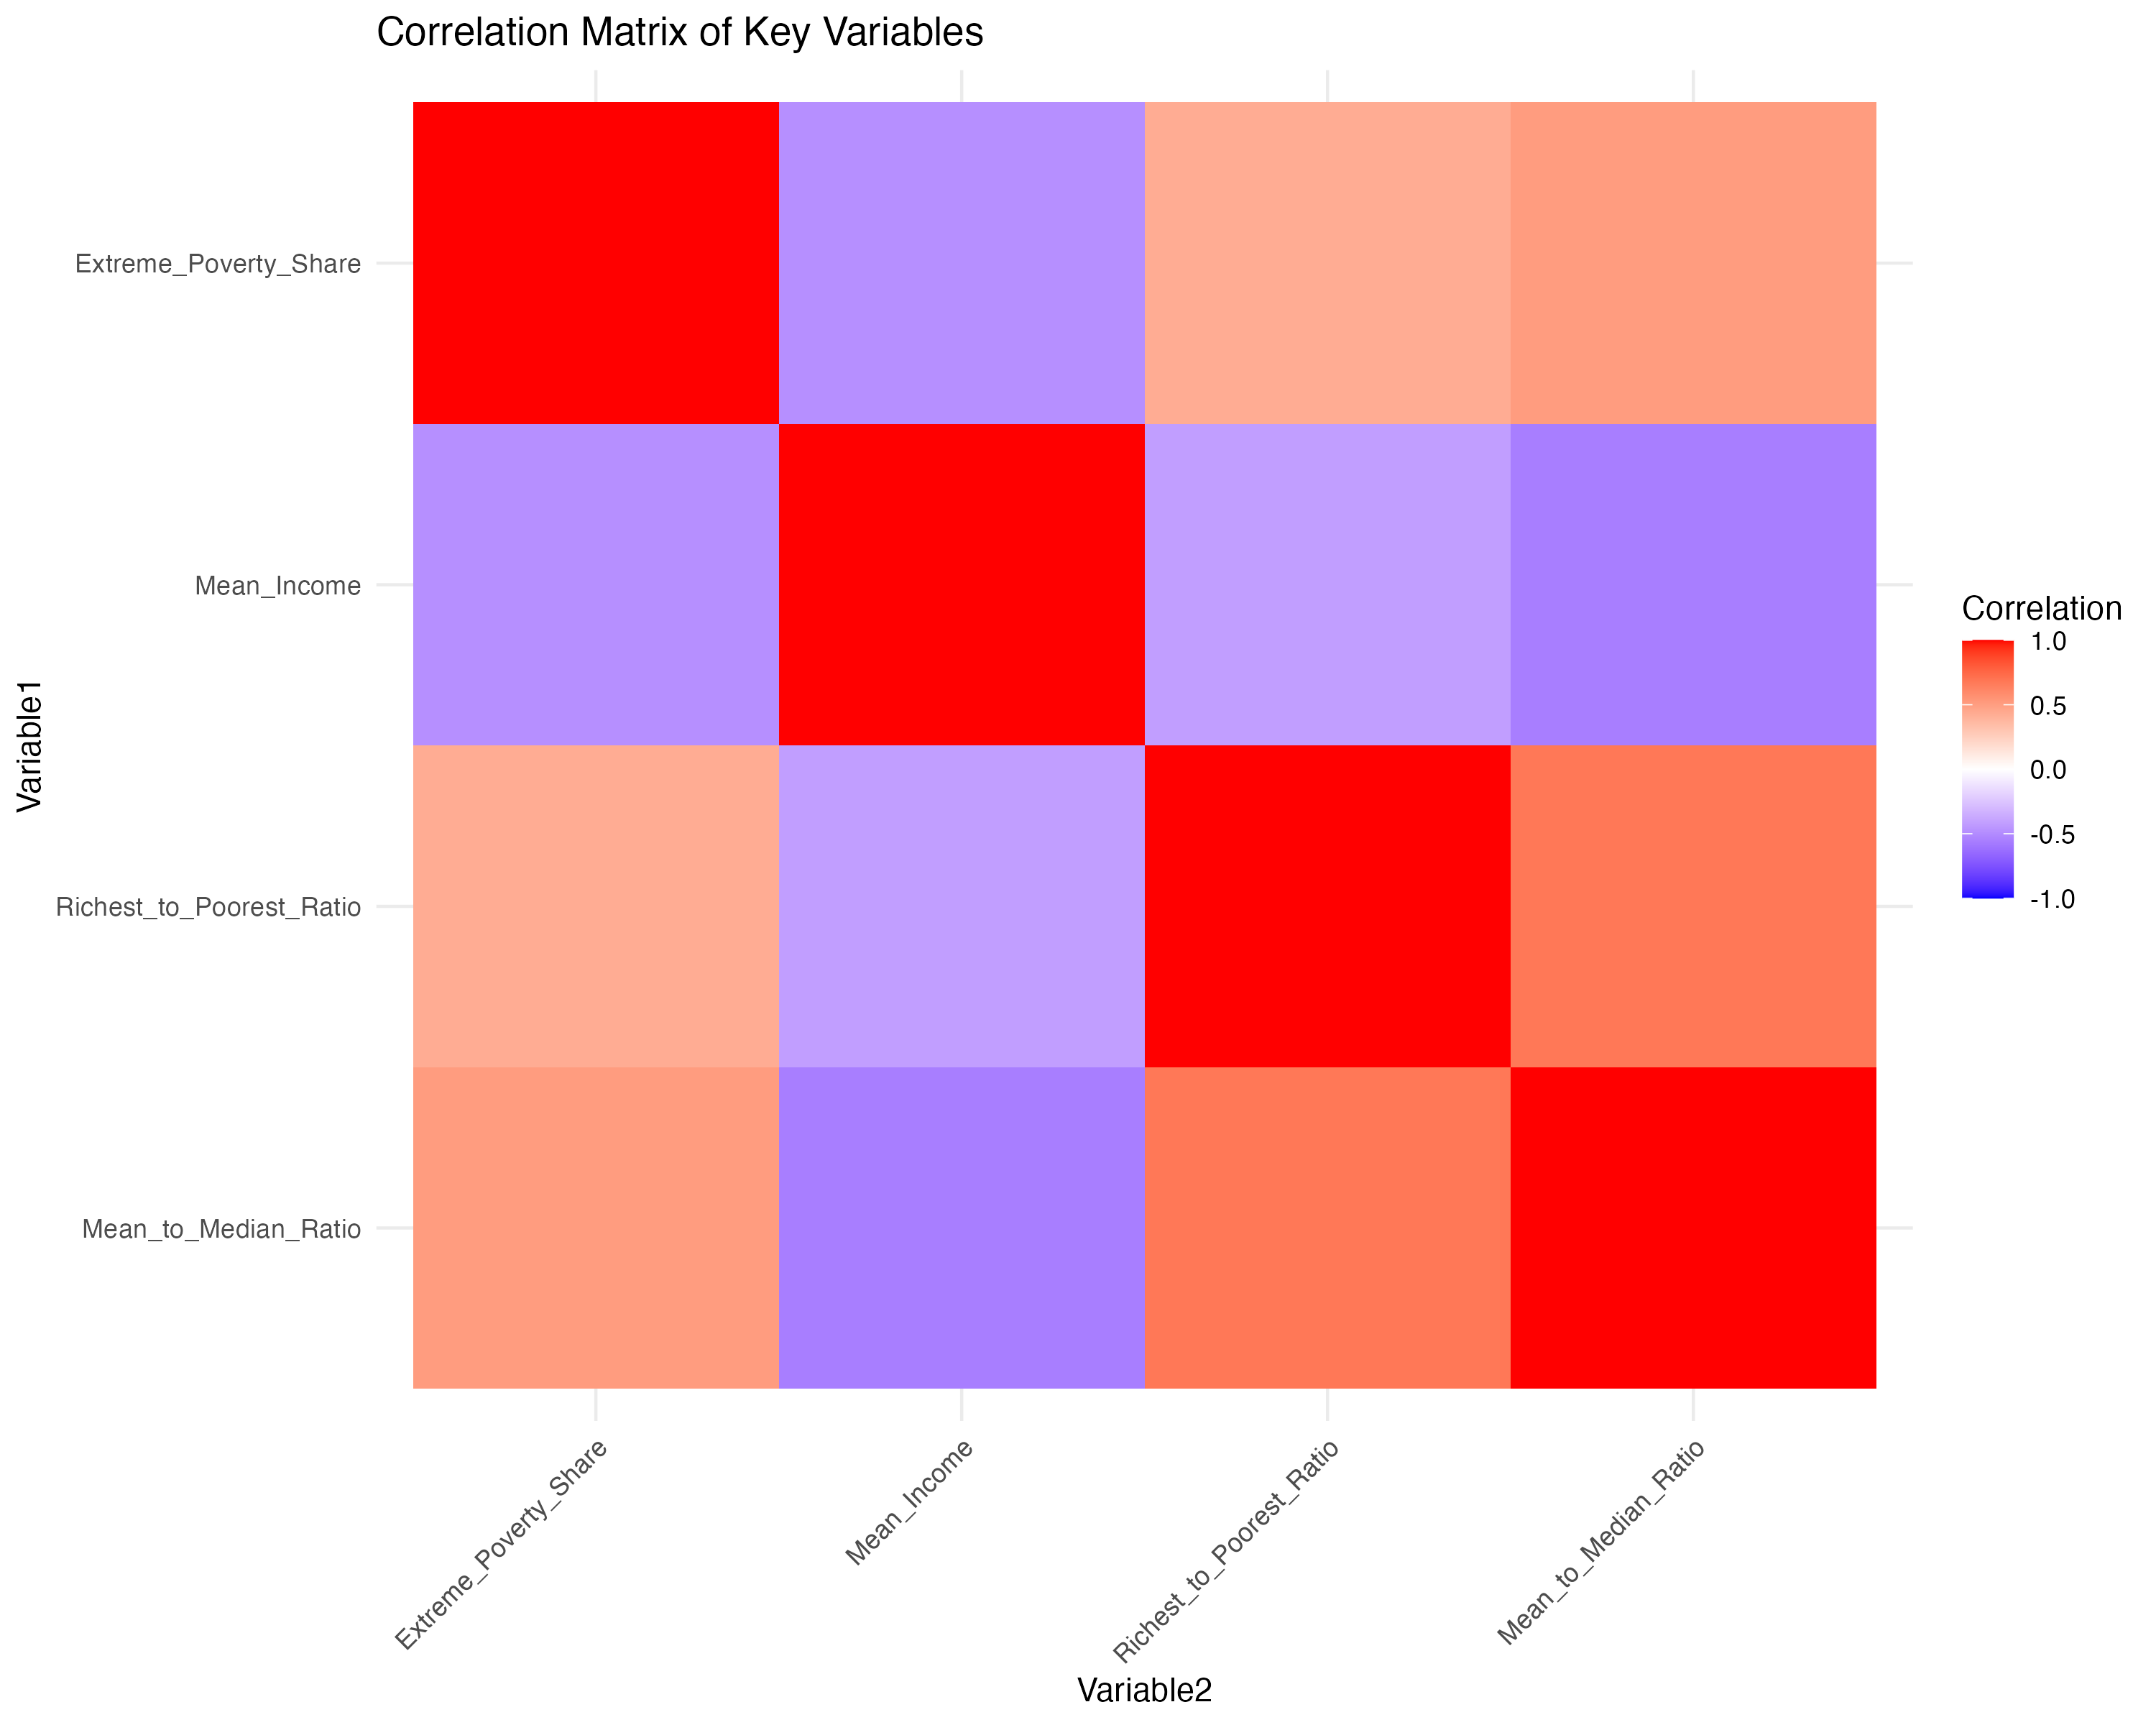
\includegraphics[width=0.8\textwidth]{../output/visualizations/correlation_heatmap.png}
    \caption{Correlation Heatmap of Key Variables}
    \end{figure}
    \item \textbf{Trend Analysis:} We applied time series techniques to analyze global and country-specific trends in income distribution and poverty rates. We used moving averages, linear and polynomial trend modeling, and Mann-Kendall trend tests to assess the significance and direction of trends.
    \begin{figure}[h]
    \centering
    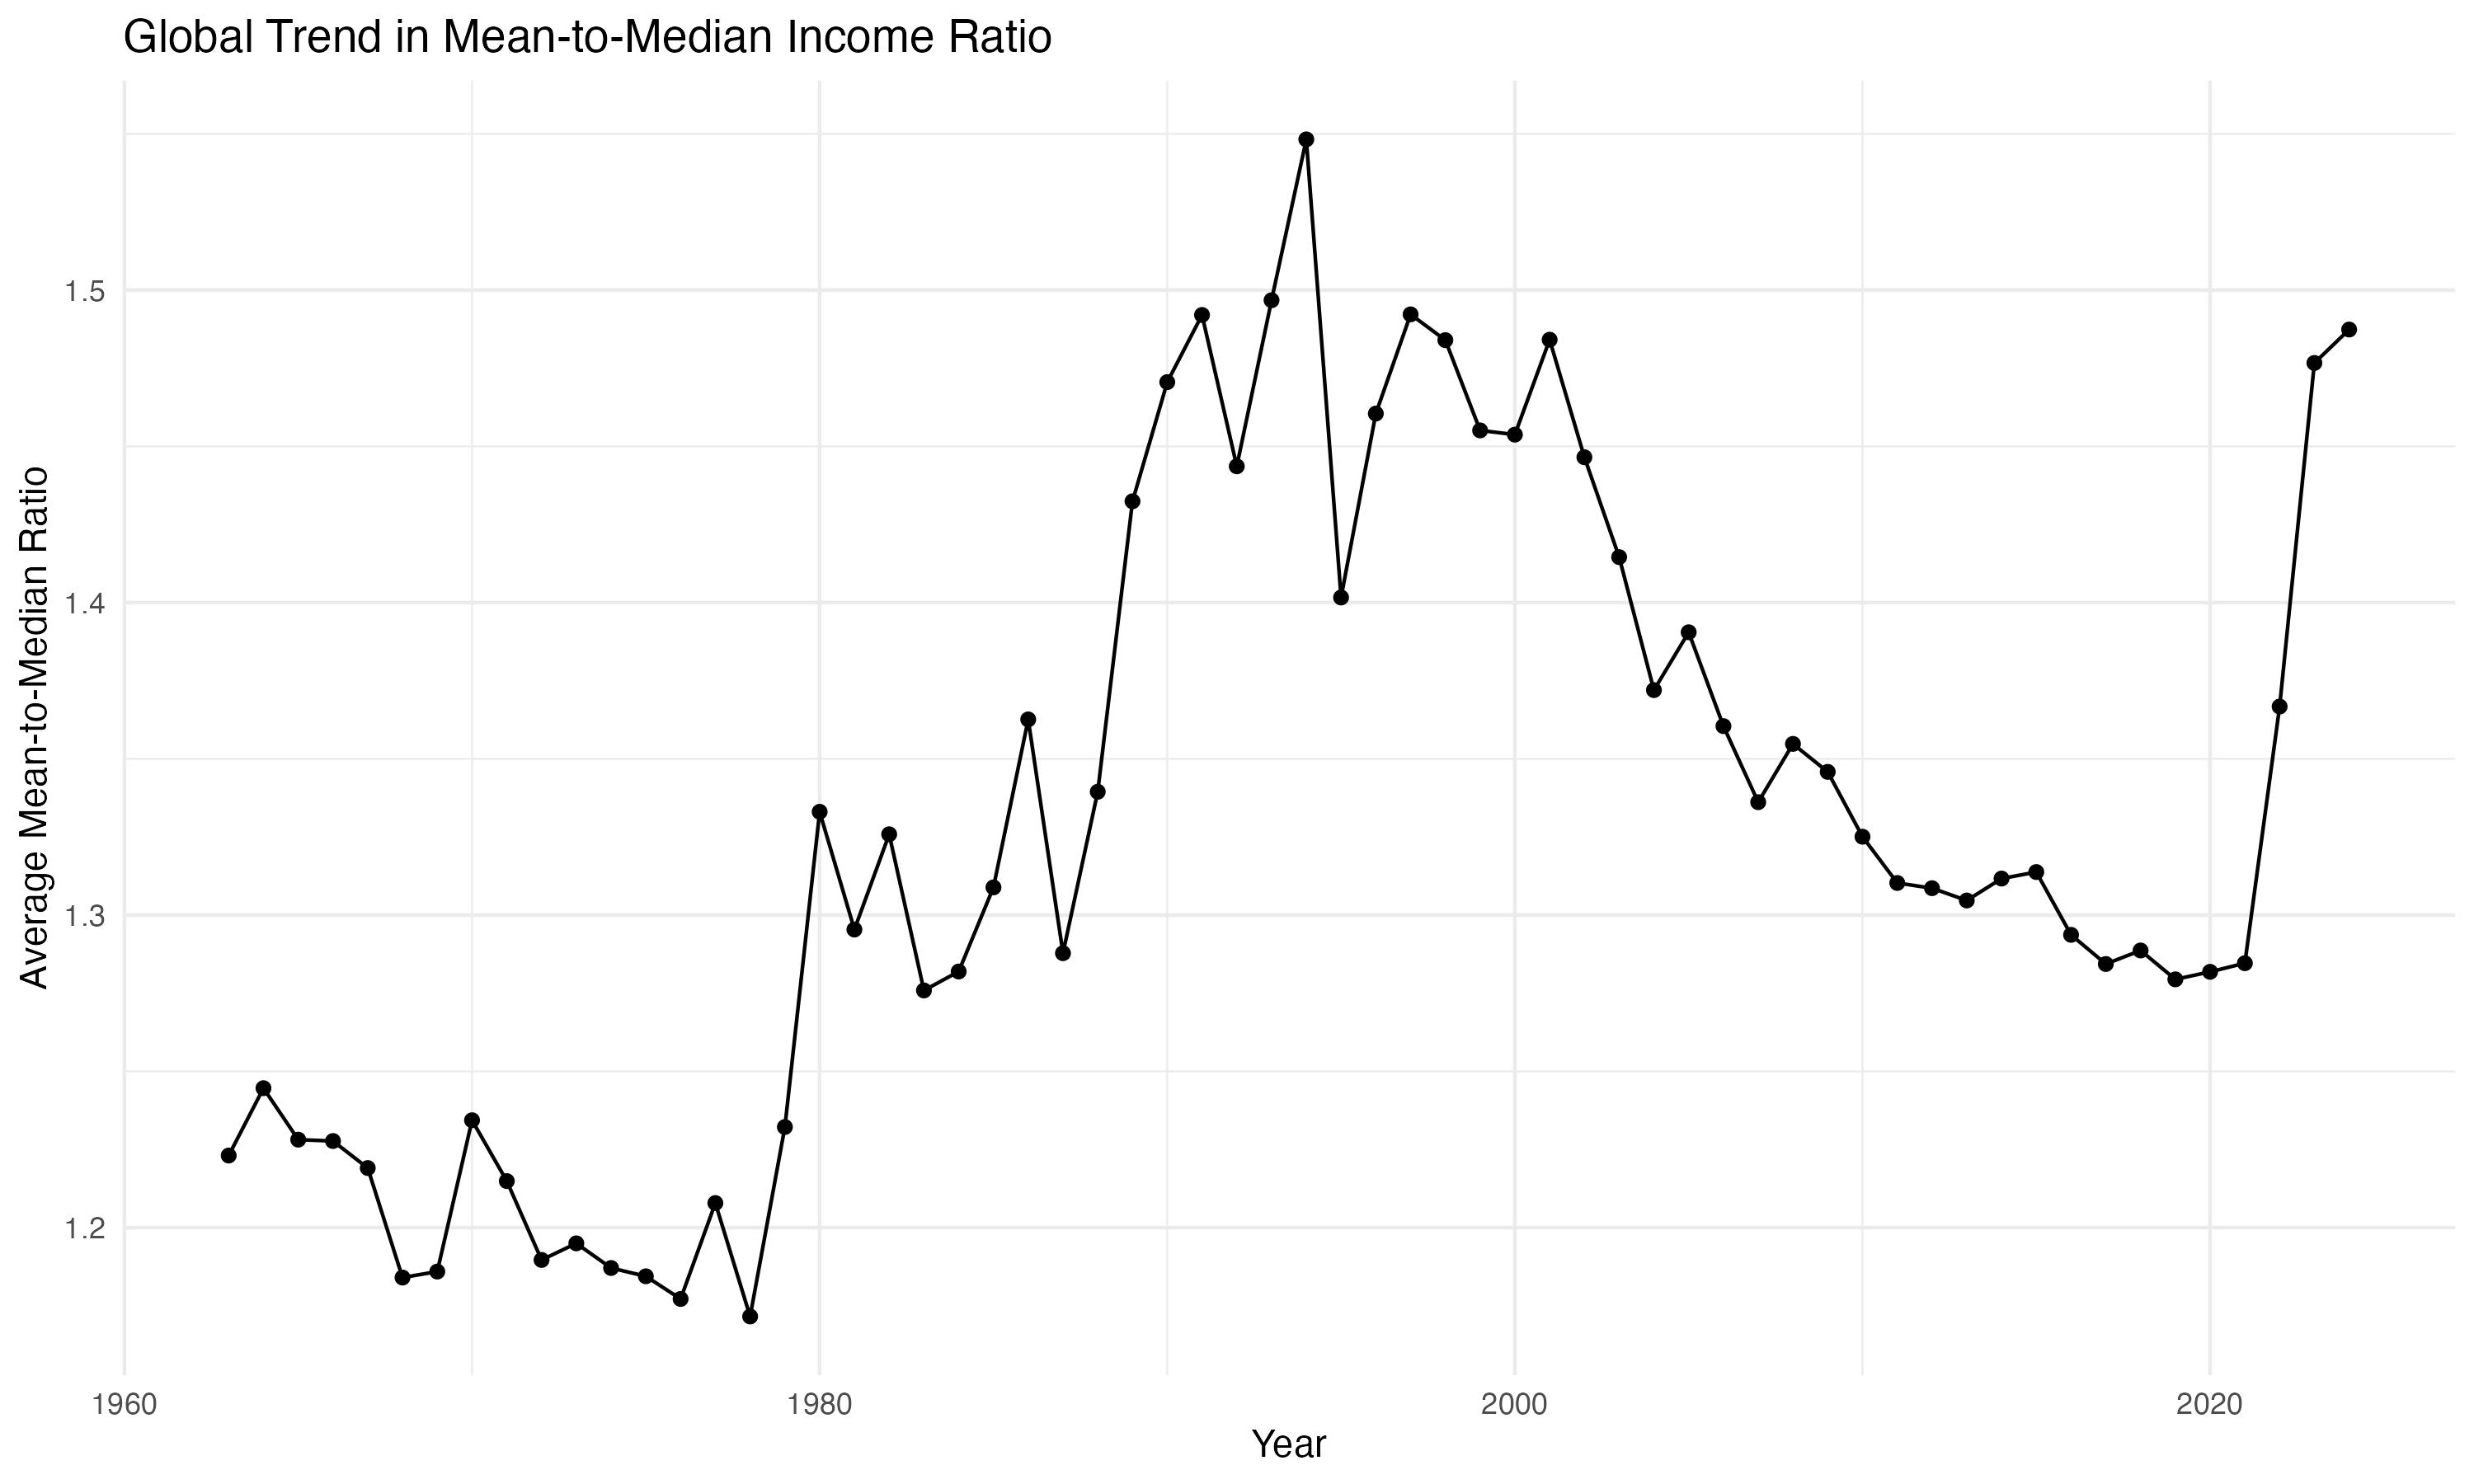
\includegraphics[width=0.8\textwidth]{../output/visualizations/mean_median_trend.png}
    \caption{Global Trend in Mean-to-Median Income Ratio}
    \end{figure}
    \item \textbf{Regional Analysis:} We grouped countries into regions (East Asia, South Asia, Europe, Latin America, Sub-Saharan Africa, and Other) and conducted analysis of variance (ANOVA) to test for significant differences in poverty rates between regions. We used Tukey's Honest Significant Difference (HSD) test for pairwise comparisons between regions.
    \begin{figure}[h]
    \centering
    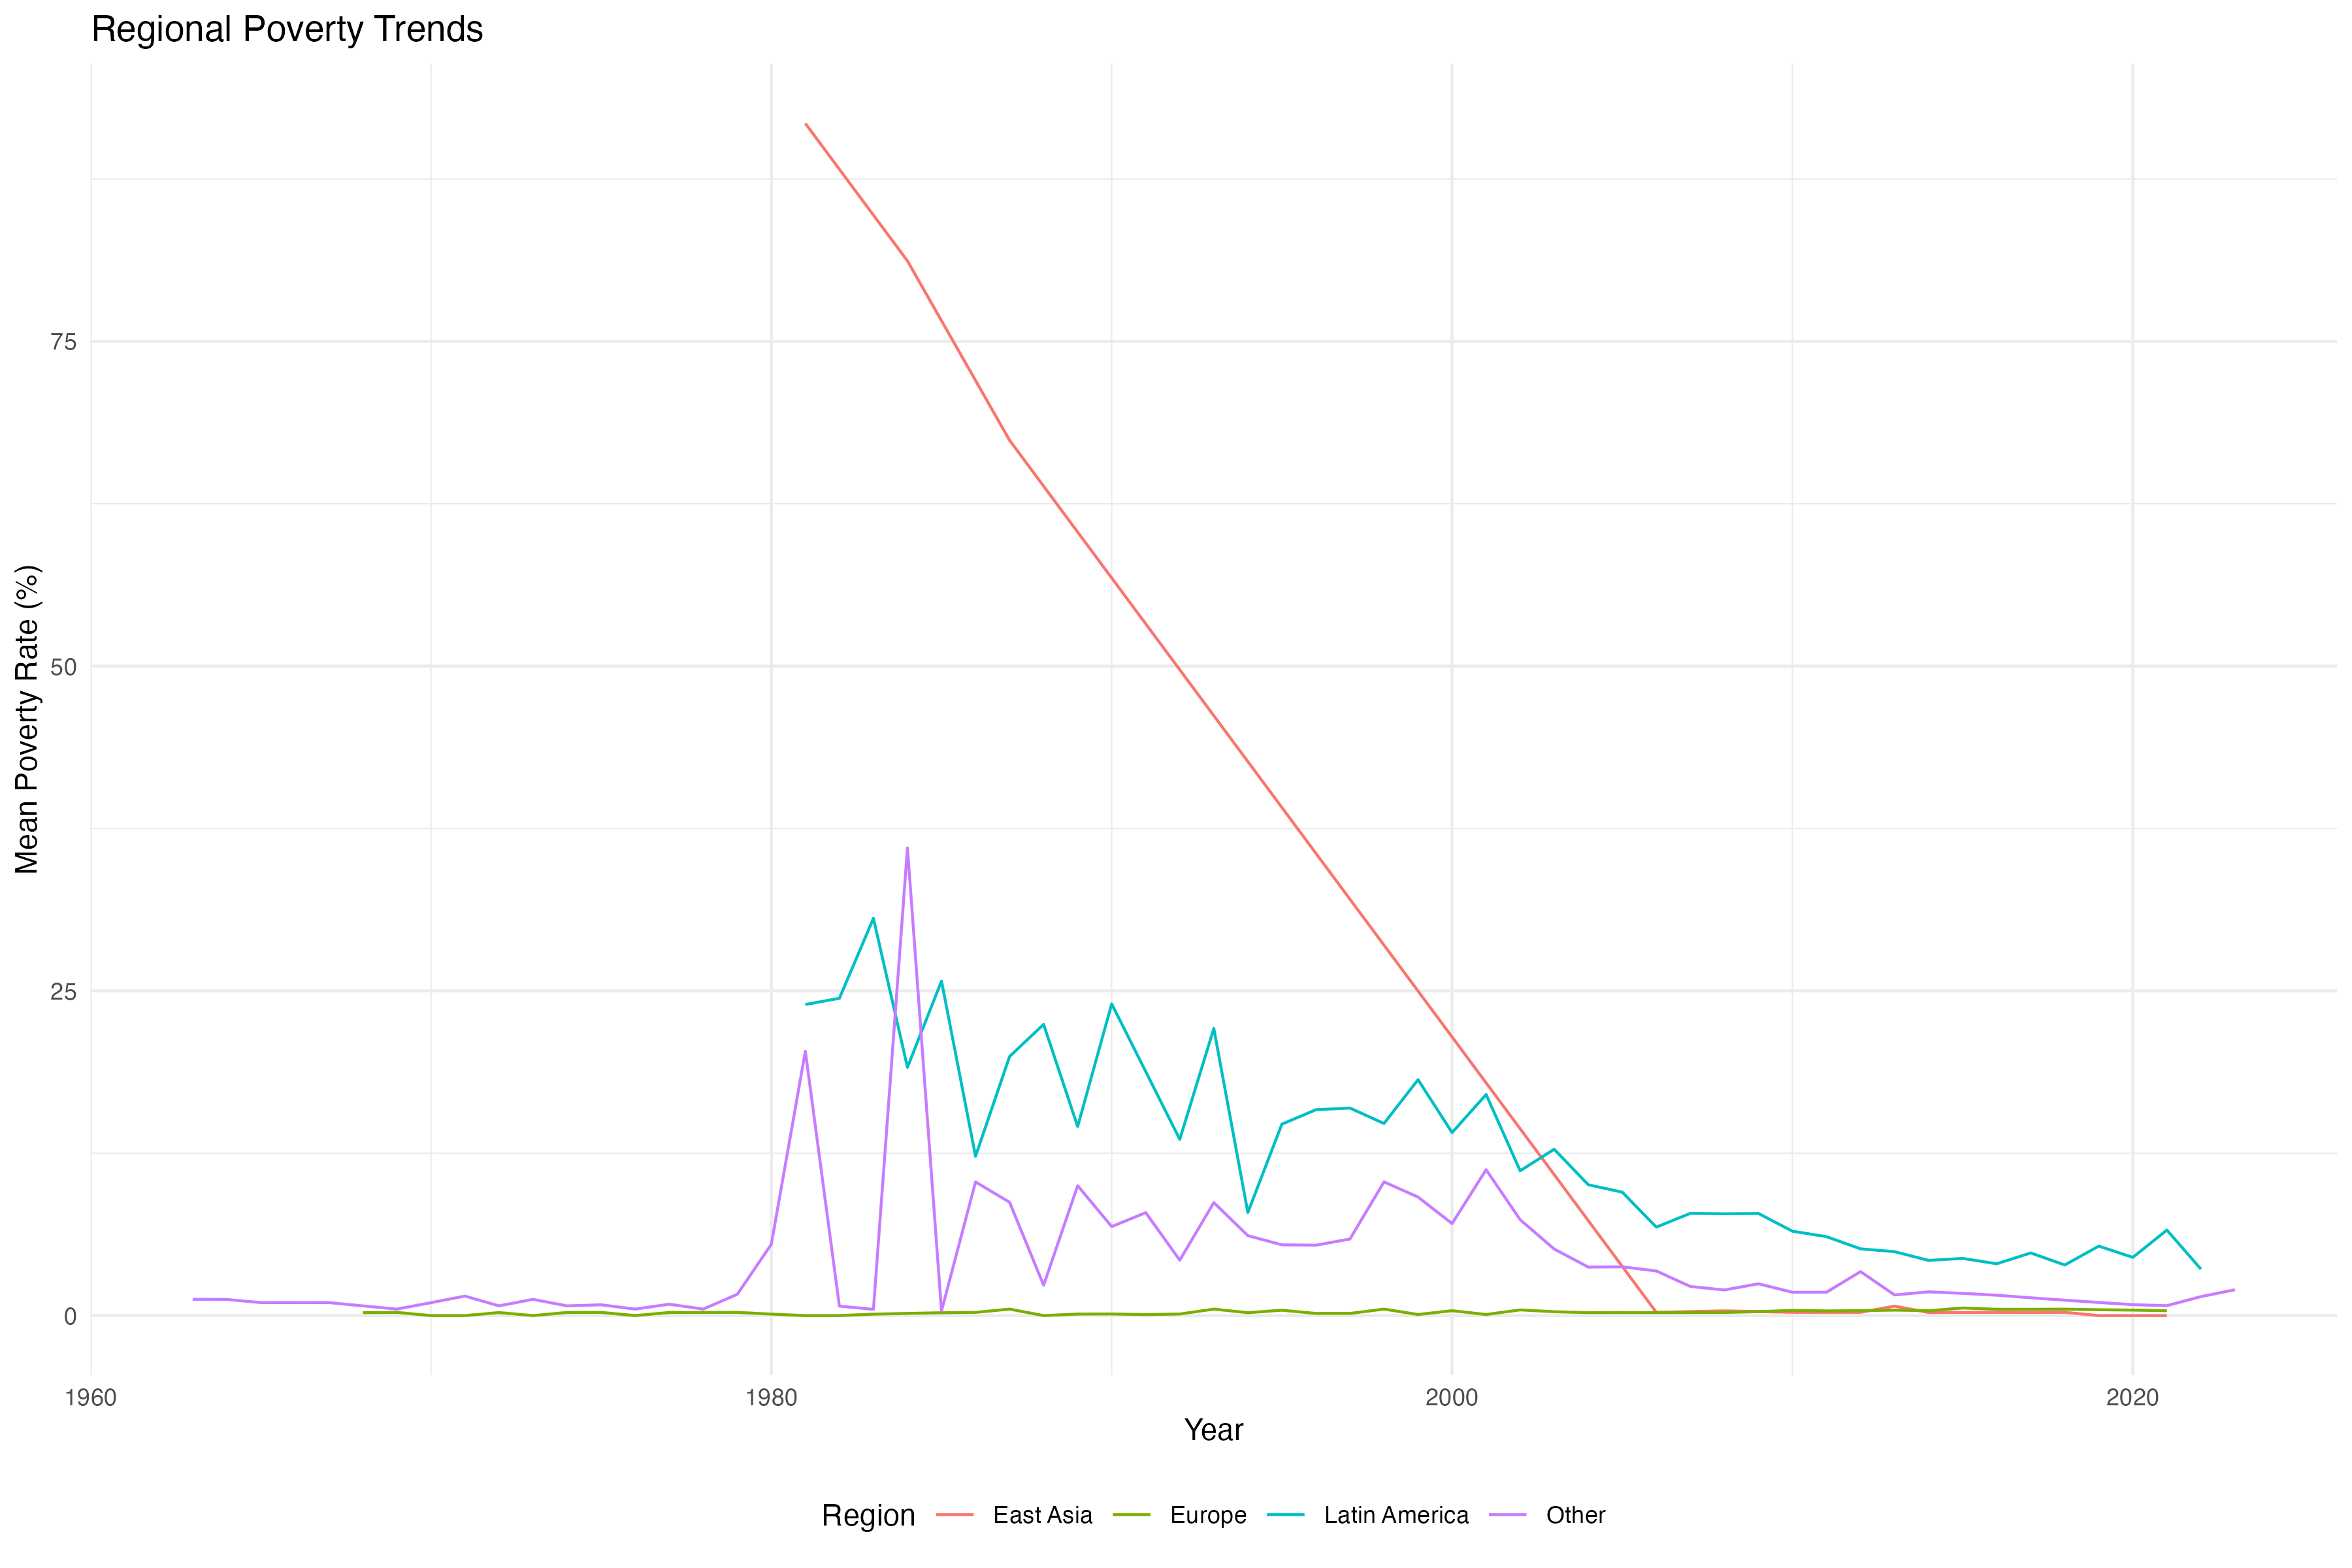
\includegraphics[width=0.8\textwidth]{../output/visualizations/regional_poverty_trends.png}
    \caption{Regional Poverty Trends}
    \end{figure}
    \item \textbf{Poverty Reduction Metrics:} To evaluate poverty reduction success, we calculated three metrics for countries with sufficient data (at least 5 data points spanning 10+ years): 
    \begin{itemize}
        \item \textbf{Absolute Reduction} = Initial Poverty Rate - Final Poverty Rate. This measures the raw percentage point decrease in poverty.
        \item \textbf{Relative Reduction} = (Initial Poverty Rate - Final Poverty Rate) / Initial Poverty Rate $\times$ 100. This measures the percentage decrease relative to the starting point, allowing comparisons between countries with different initial poverty levels.
        \item \textbf{Annual Reduction Rate} = Absolute Reduction / Year Range. This measures the average yearly progress, enabling comparisons between countries with different measurement periods.
    \end{itemize}
    \begin{figure}[h]
    \centering
    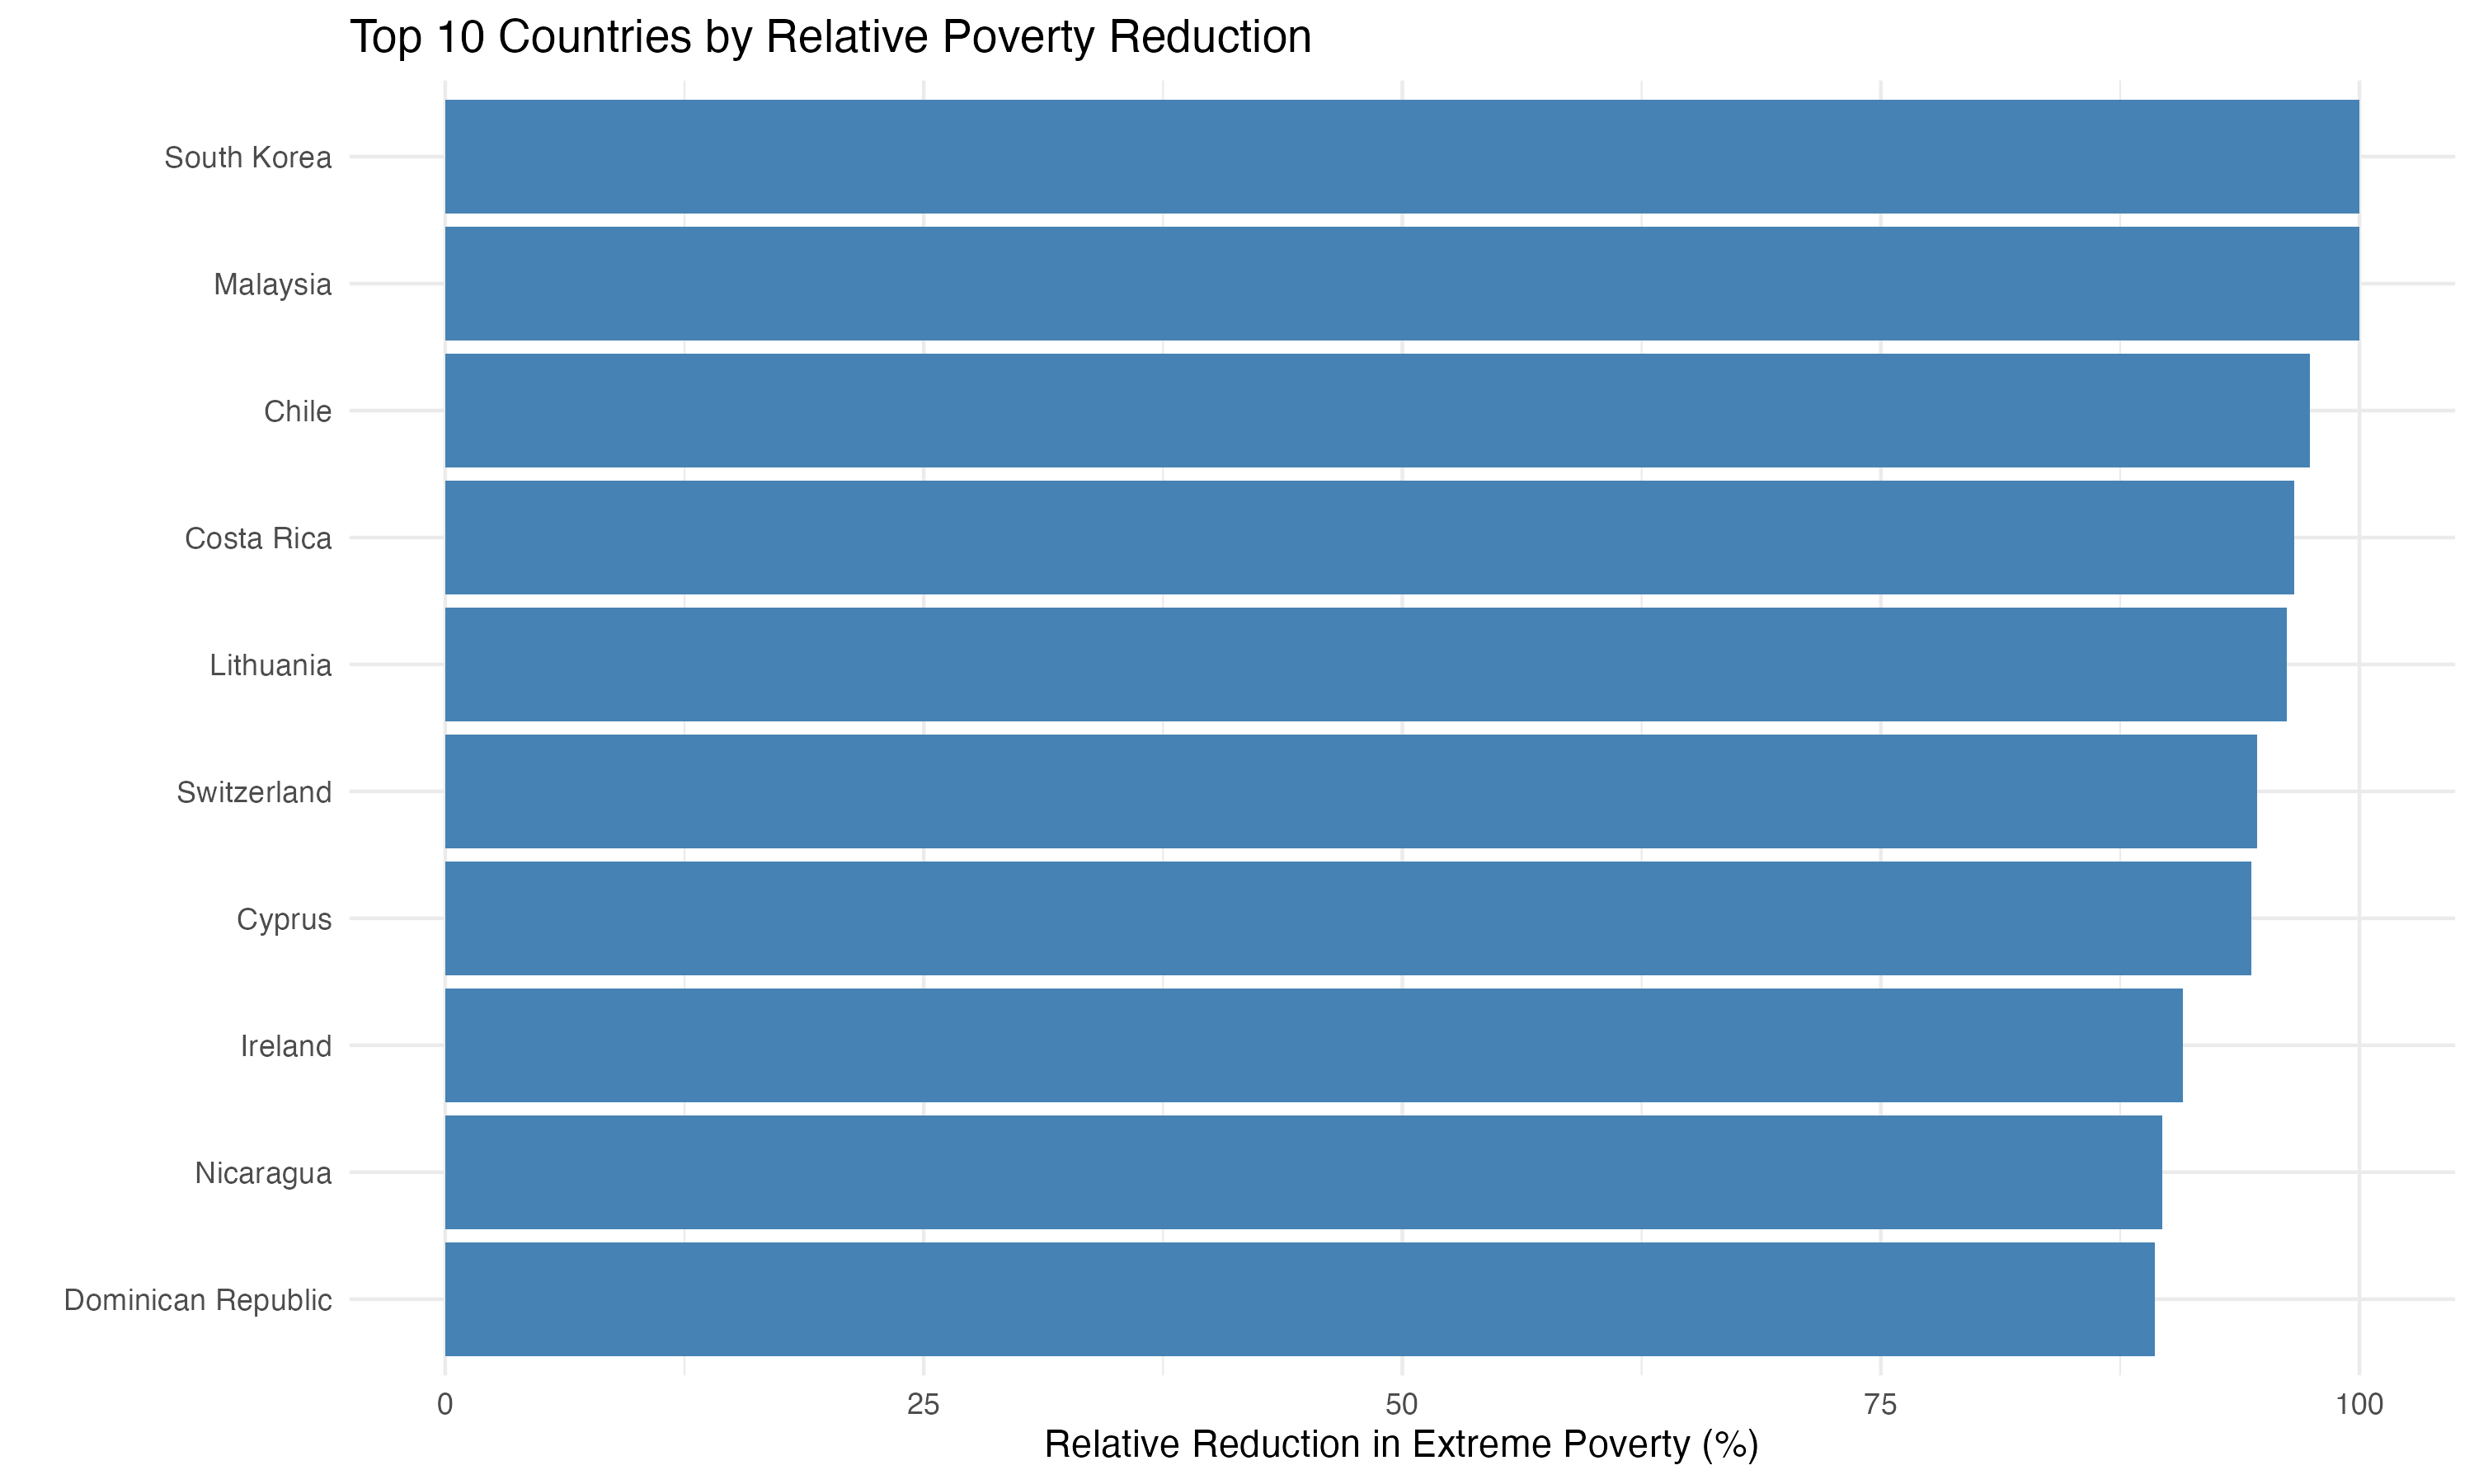
\includegraphics[width=0.8\textwidth]{../output/visualizations/top_poverty_reducers.png}
    \caption{Top Countries by Relative Poverty Reduction}
    \end{figure}
    \item \textbf{Regression Modeling:} We developed four nested regression models to examine the relationship between income, inequality, and poverty: 
    \begin{itemize}
        \item \textbf{Model 1:} Extreme\_Poverty\_Share = $\beta_0$ + $\beta_1\log($Mean\_Income$) + \epsilon$. This baseline model examines the relationship between income levels and poverty rates.
        \item \textbf{Model 2:} Extreme\_Poverty\_Share = $\beta_0$ + $\beta_1$Richest\_to\_Poorest\_Ratio + $\epsilon$. This model isolates the relationship between inequality and poverty.
        \item \textbf{Model 3:} Extreme\_Poverty\_Share = $\beta_0$ + $\beta_1\log($Mean\_Income$) + \beta_2$Richest\_to\_Poorest\_Ratio + $\epsilon$. This additive model examines the combined effects of income and inequality.
        \item \textbf{Model 4:} Extreme\_Poverty\_Share = $\beta_0$ + $\beta_1\log($Mean\_Income$) + \beta_2$Richest\_to\_Poorest\_Ratio + $\beta_3(\log($Mean\_Income$) \times$ Richest\_to\_Poorest\_Ratio$) + \beta_4$Mean\_to\_Median\_Ratio + $\epsilon$. This interaction model tests whether the relationship between income and poverty depends on inequality levels.
    \end{itemize}
    \begin{figure}[h]
    \centering
    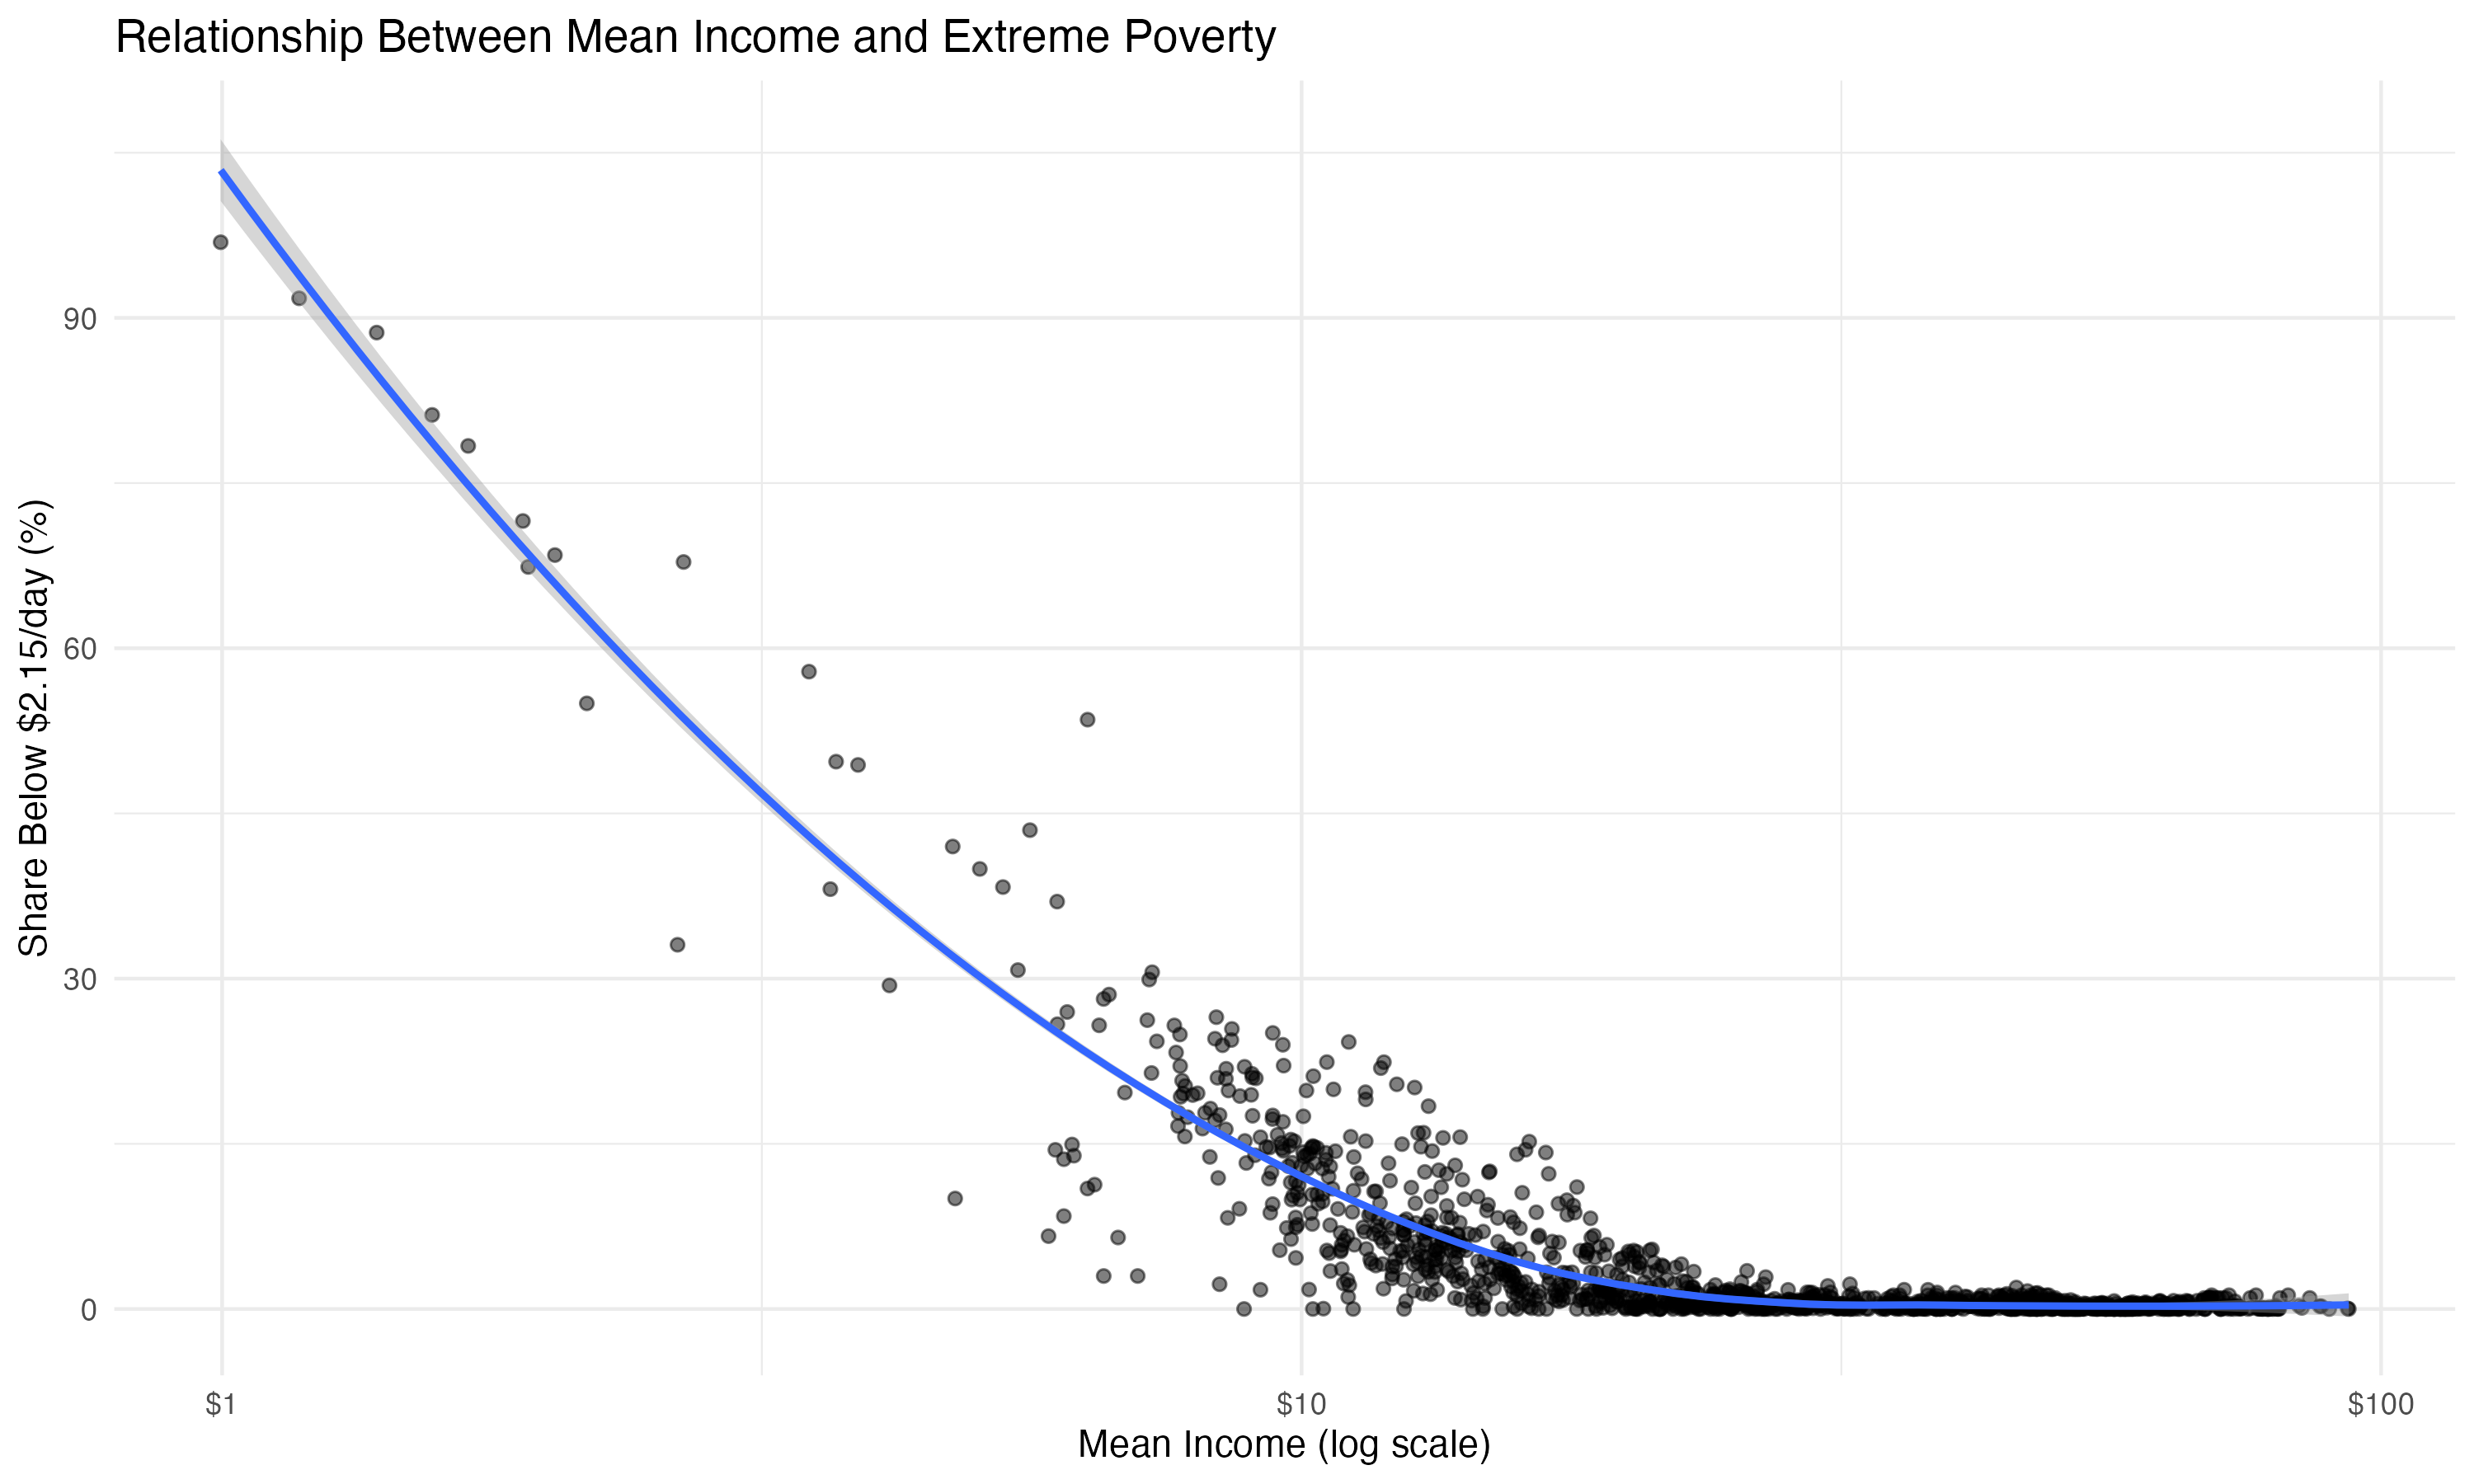
\includegraphics[width=0.8\textwidth]{../output/visualizations/income_poverty_relationship.png}
    \caption{Relationship Between Mean Income and Extreme Poverty}
    \end{figure}
    \item \textbf{Time Series Decomposition and Forecasting:} We decomposed global poverty trends into trend, seasonal, and random components using moving averages. We then used ARIMA modeling to forecast future poverty rates based on historical patterns.
    \begin{figure}[h]
    \centering
    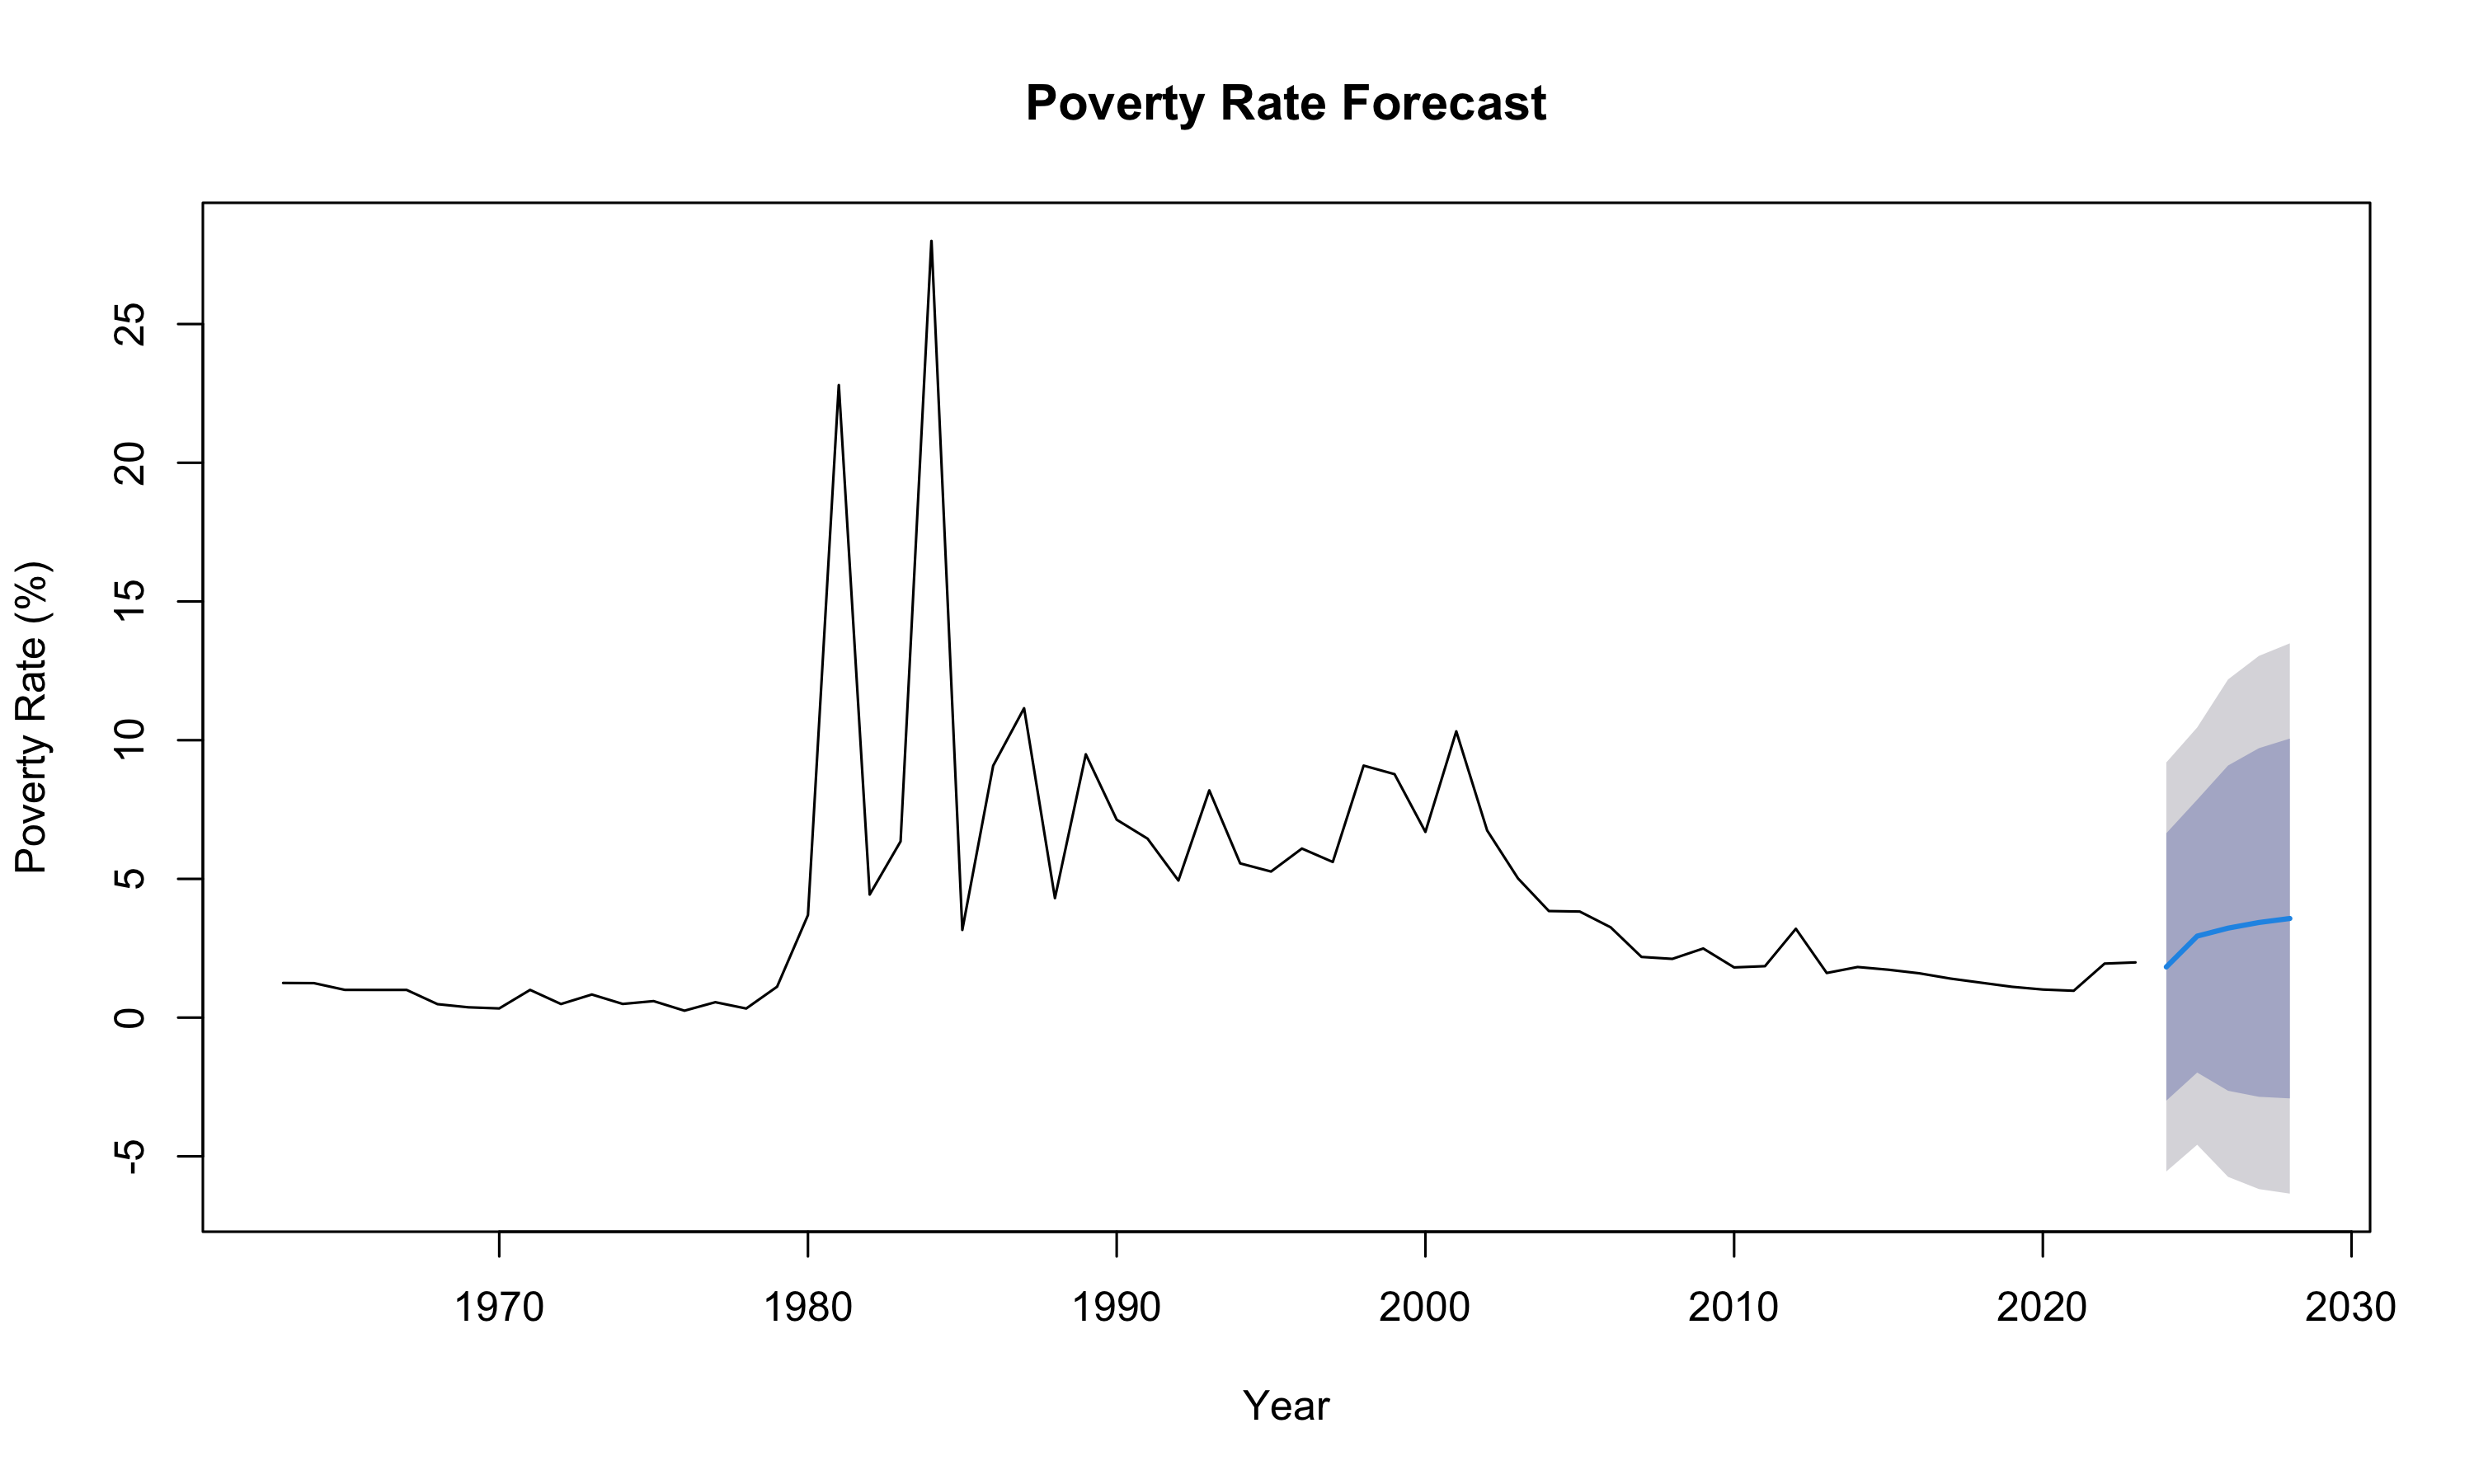
\includegraphics[width=0.8\textwidth]{../output/visualizations/poverty_forecast.png}
    \caption{Poverty Rate Forecast}
    \end{figure}
\end{enumerate}

All analyses were conducted using R version 4.2.0, with packages including dplyr, ggplot2, tidyr, forecast, tseries, lmtest, and car.

\section{Analysis and Results}\label{sec:results}

\subsection{Hypothesis Testing Framework}
Our research was guided by four primary hypotheses:
\begin{enumerate}
    \item \textbf{H1:} Countries with lower income inequality (measured by mean-to-median ratio) will show greater poverty reduction over time
    \begin{itemize}
        \item H$_0$: There is no relationship between income inequality and poverty reduction rates
        \item H$_1$: Countries with lower income inequality experience greater poverty reduction over time
    \end{itemize}
    \item \textbf{H2:} The relationship between economic growth and poverty reduction is moderated by income distribution patterns
    \begin{itemize}
        \item H$_0$: The effect of economic growth on poverty reduction is the same regardless of income distribution
        \item H$_1$: The poverty-reducing effect of economic growth varies based on income distribution patterns
    \end{itemize}
    \item \textbf{H3:} Regional differences in poverty reduction success are statistically significant
    \begin{itemize}
        \item H$_0$: There are no significant differences in poverty reduction success between regions
        \item H$_1$: Different regions show significantly different poverty reduction patterns
    \end{itemize}
    \item \textbf{H4:} The poorest decile's growth rate is a significant predictor of overall poverty reduction
    \begin{itemize}
        \item H$_0$: Growth rates of the poorest decile are not significantly related to overall poverty reduction
        \item H$_1$: Higher growth rates for the poorest decile predict greater overall poverty reduction
    \end{itemize}
\end{enumerate}

The results of our testing for these hypotheses are integrated into the relevant sections below.

\subsection{Correlation Analysis}
Our correlation analysis revealed meaningful relationships between income, inequality, and poverty metrics. The Pearson correlation between mean income and extreme poverty rate was -0.481, indicating a moderate negative relationship where higher income is associated with lower poverty rates. The correlation between the richest-to-poorest ratio and extreme poverty was 0.428, showing that higher inequality is associated with higher poverty rates.

Converting these correlation coefficients to coefficients of determination (r$^2$) helps quantify the proportion of variance shared between variables. For example, the correlation between mean income and extreme poverty (r = -0.481) yields r$^2$ = 0.231, indicating that mean income explains approximately 23.1\% of the variance in poverty rates. Similarly, the richest-to-poorest ratio (r = 0.428, r$^2$ = 0.183) explains 18.3\% of the variance in poverty rates.

The mean-to-median ratio showed a stronger correlation with poverty (0.508, r$^2$ = 0.258) than the richest-to-poorest ratio, suggesting that income distribution skewness may be a more important factor in poverty than the gap between the richest and poorest deciles. Perhaps most notably, the Gini coefficient showed the strongest correlation with extreme poverty (0.531, r$^2$ = 0.282), confirming its value as a standard measure of inequality in poverty research.

When examining Spearman rank correlations, the relationship between inequality and poverty appeared even stronger (0.805 for richest-to-poorest ratio, r$^2$ = 0.648), indicating that the relationship may be non-linear. This stronger Spearman correlation suggests that inequality explains nearly 65\% of the variance in poverty ranks rather than absolute values.

Partial correlation analysis revealed that even when controlling for other factors, the relationship between mean income and poverty (-0.271) and between inequality and poverty (0.120 for richest-to-poorest ratio) remained significant.

These correlation results provide initial support for our first hypothesis (H1), showing a significant relationship between inequality metrics and poverty rates.

\subsection{Global Trends in Income Distribution and Poverty}
Our analysis of global trends revealed several important patterns:
\begin{enumerate}
    \item \textbf{Mean-to-Median Income Ratio:} The global average mean-to-median ratio has decreased from 1.41 to 1.32 over the period covered by our data, suggesting a modest global trend toward more equal distribution.
    \item \textbf{Richest-to-Poorest Decile Ratio:} Similarly, the richest-to-poorest decile ratio has decreased from 7.73 to 6.54, indicating a narrowing of the gap between the top and bottom of the income distribution globally.
    \item \textbf{Gini Coefficient:} Our data shows a gradual decline in the average global Gini coefficient from 0.41 in the 1970s to 0.36 by 2022. This 12.2\% decrease aligns with the trends observed in our other inequality metrics, providing robust evidence of a modest global reduction in income inequality.
    \item \textbf{Extreme Poverty:} The share of population living below \$2.15 per day has shown a decreasing trend over time, though with periods of stagnation and even increases during economic crises.
    \item \textbf{Regional Convergence:} We observed a convergence in poverty rates across regions, with the highest-poverty regions showing the most significant reductions over time.
\end{enumerate}

Time series decomposition of the global poverty trend revealed that the trend component explained most of the variation in poverty rates, with a relatively small random component. Mann-Kendall trend analysis indicated a slightly increasing trend in global poverty rates (Sen's slope = 0.009 units per year), though this trend was not statistically significant (p = 0.563).

When fitting different trend models, we found that a polynomial model (adjusted R$^2$ = 0.254) outperformed a linear model (adjusted R$^2$ = -0.017), indicating a non-linear pattern in global poverty trends, with faster reduction in earlier periods and slower progress in recent years.

\begin{figure}[h]
\centering
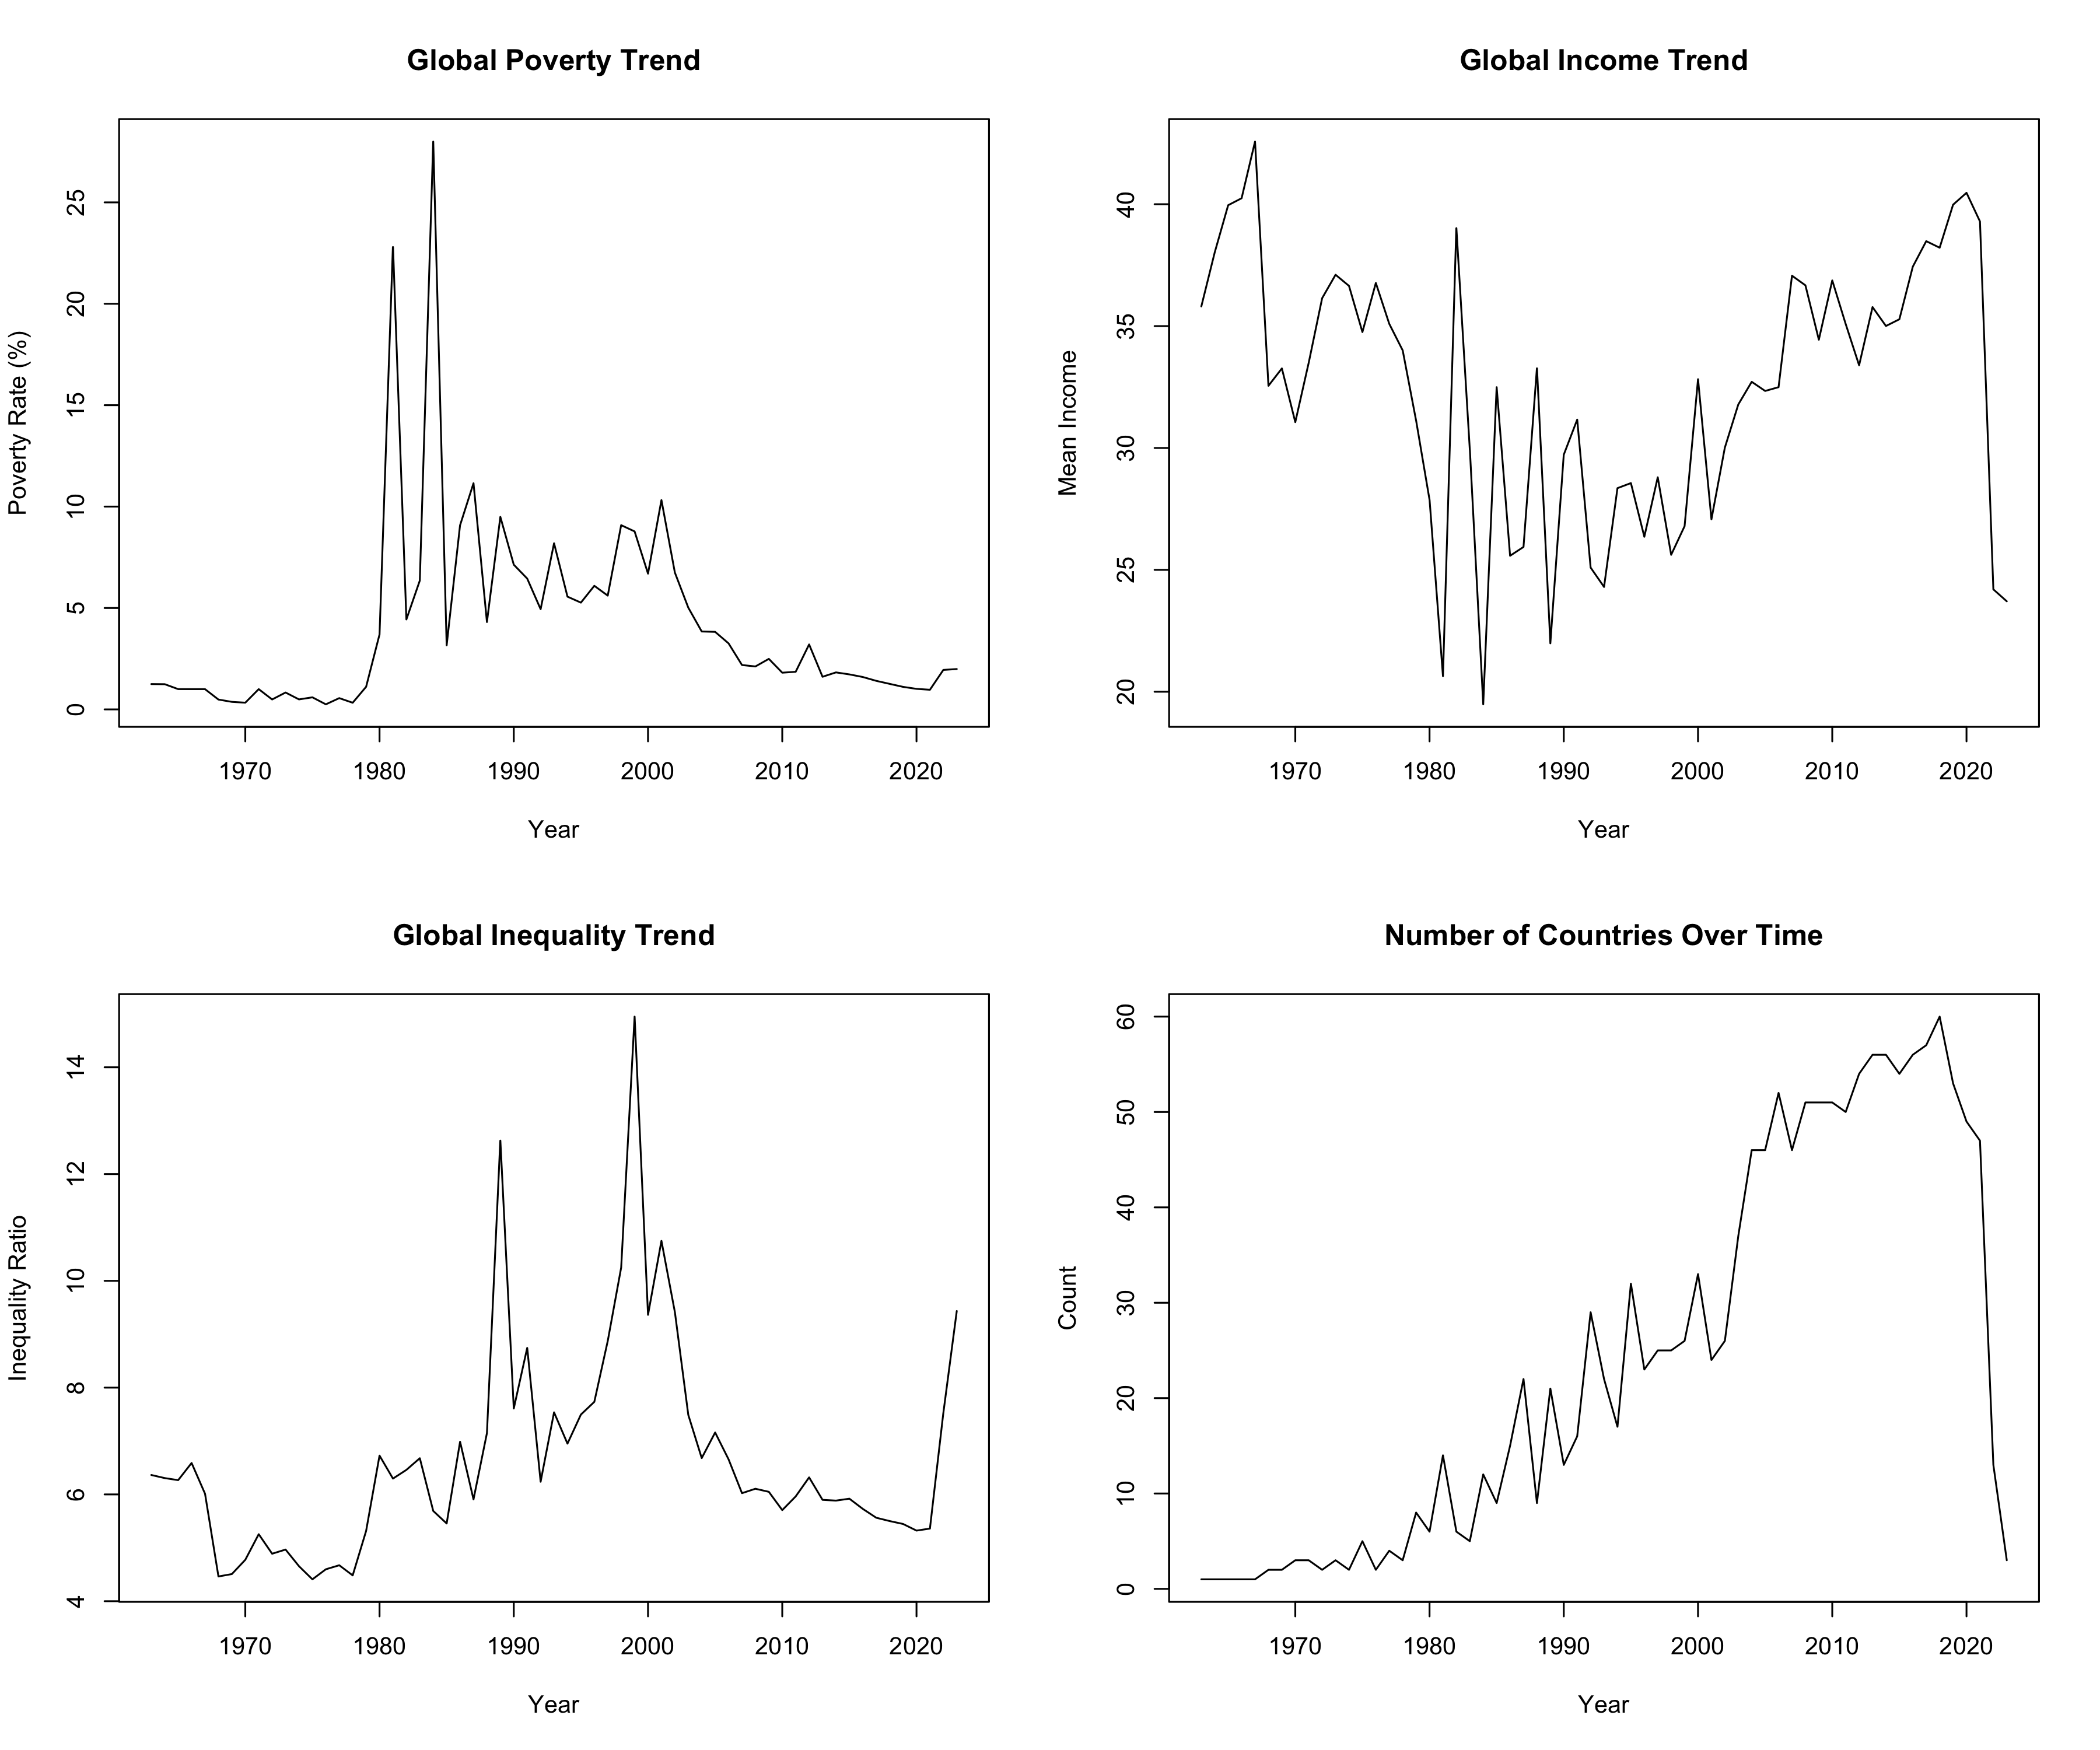
\includegraphics[width=0.8\textwidth]{../output/visualizations/global_trends.png}
\caption{Global Trends in Key Variables}
\end{figure}

\begin{figure}[h]
\centering
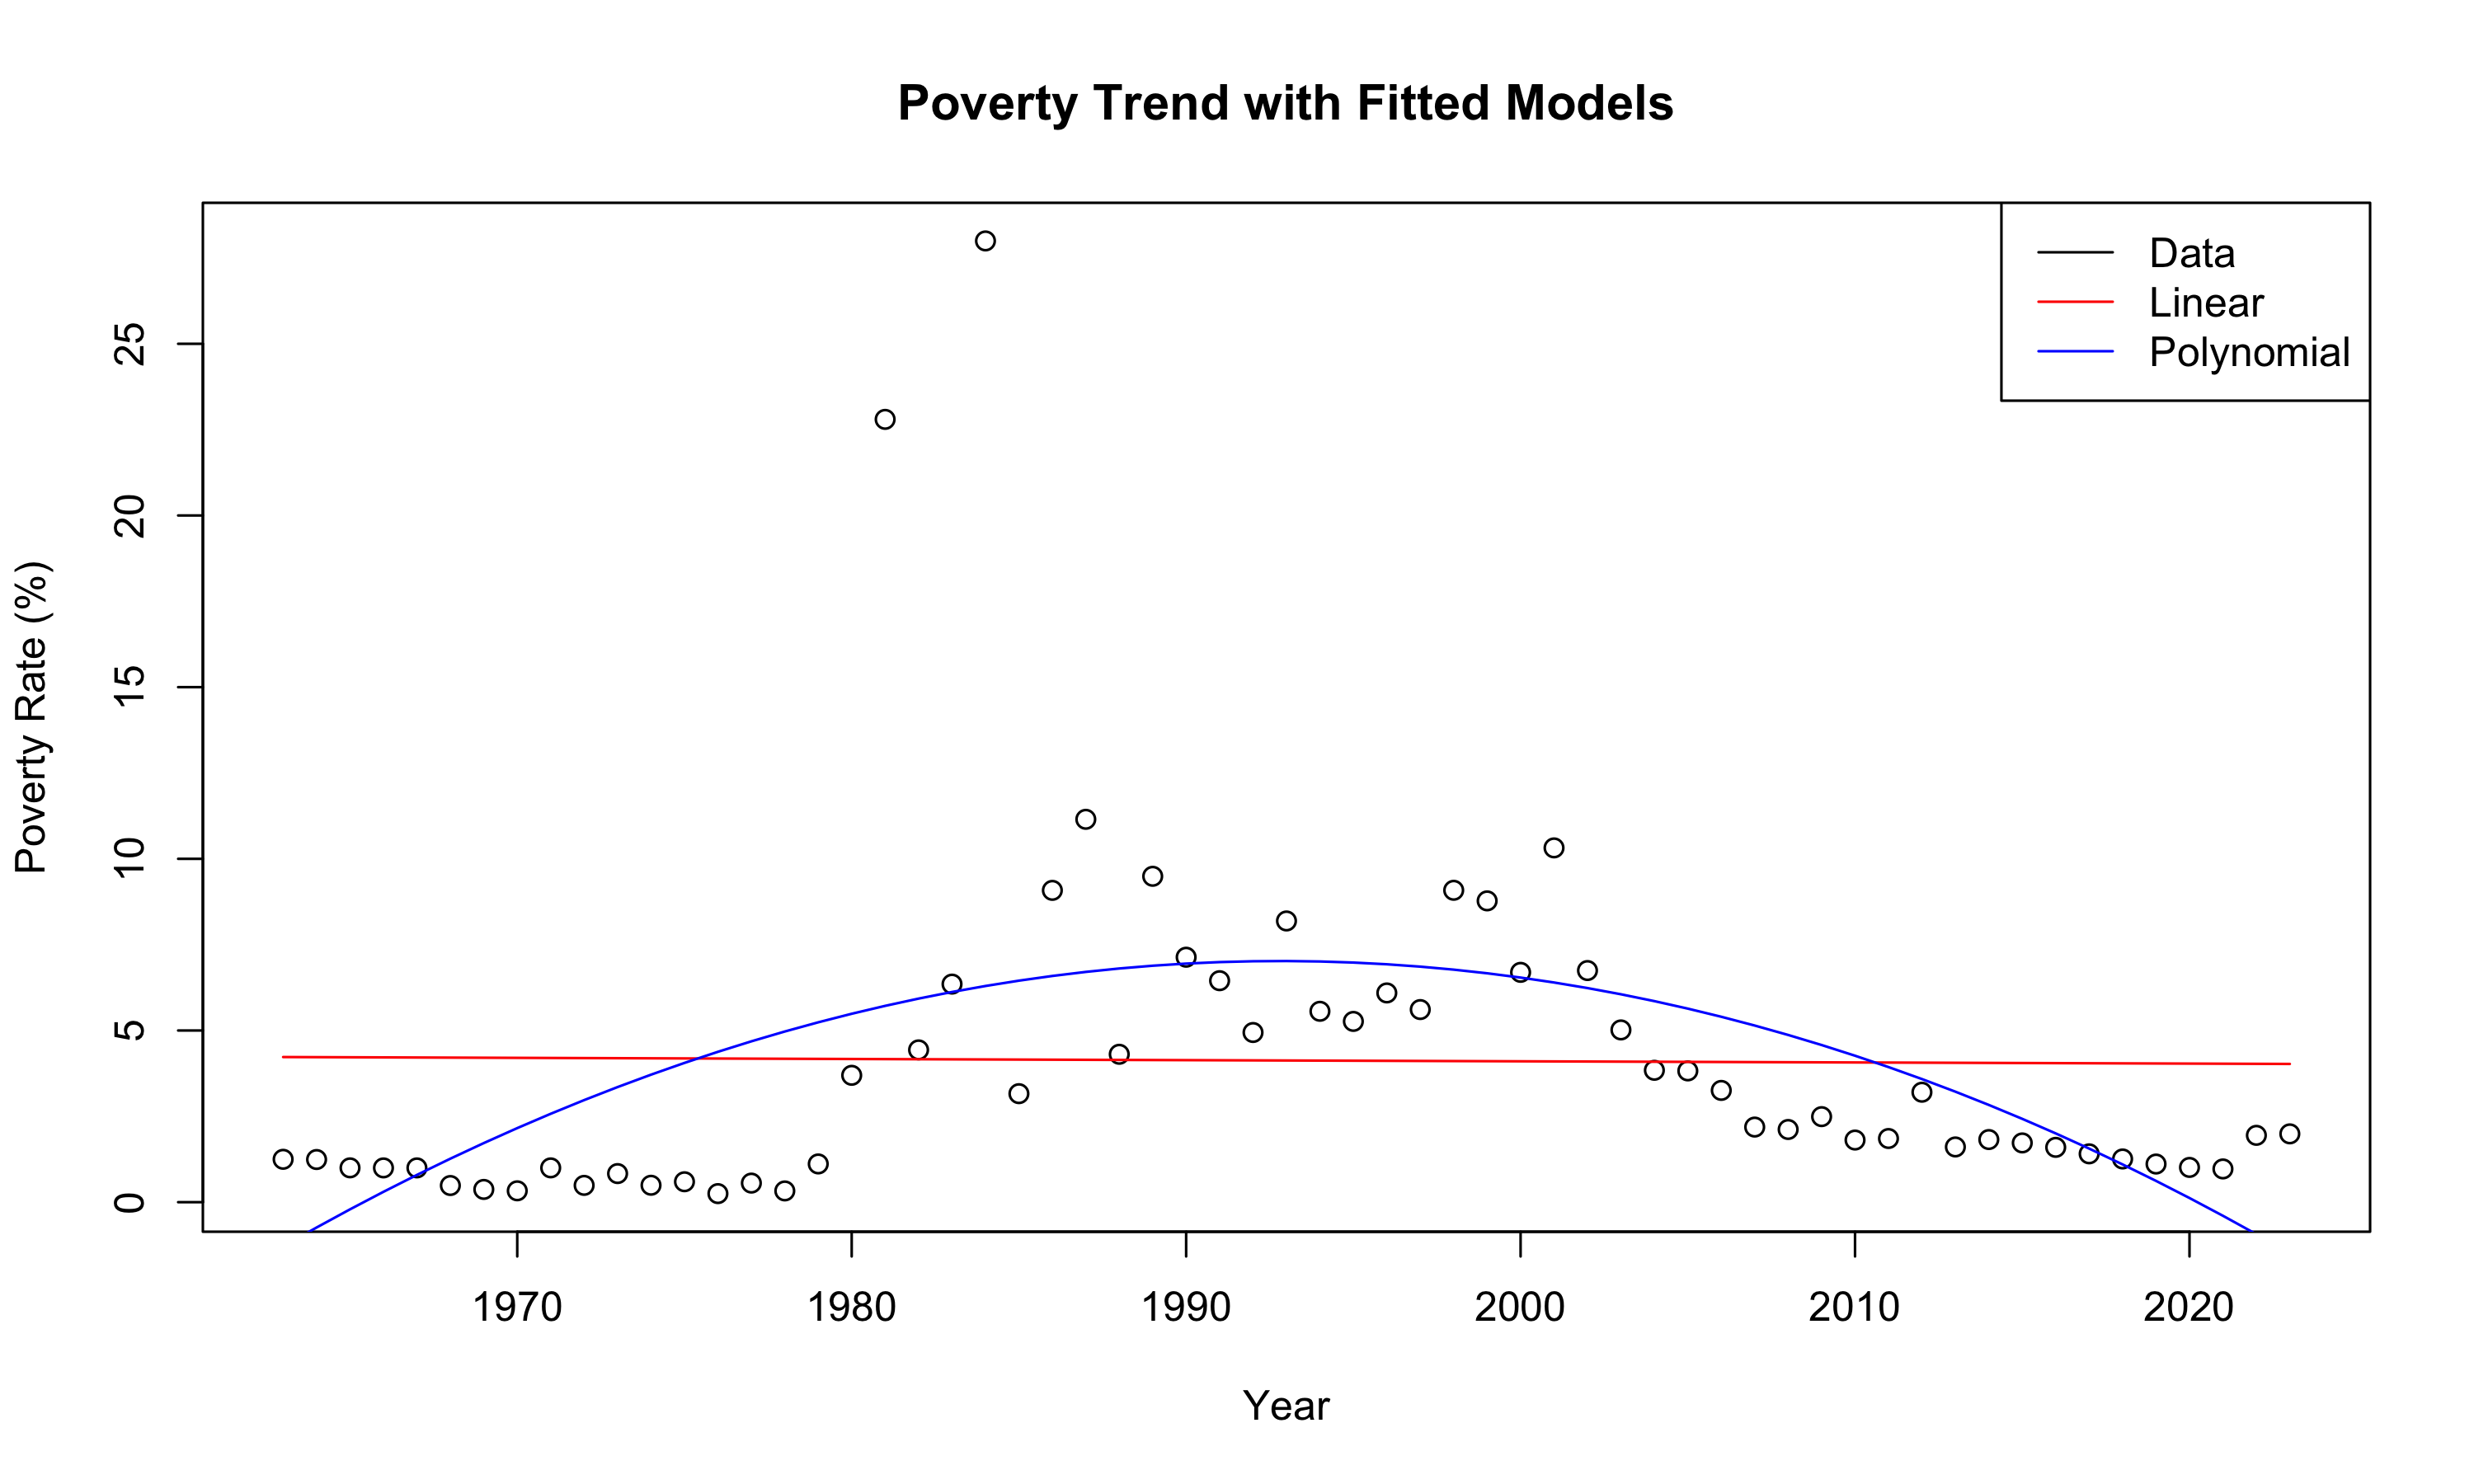
\includegraphics[width=0.8\textwidth]{../output/visualizations/trend_fits.png}
\caption{Trend Model Fits}
\end{figure}

\subsection{Country-Specific Patterns}
Our analysis of country-specific trends revealed fascinating patterns in the relationship between income distribution and poverty:
\begin{enumerate}
    \item \textbf{United States:} The mean-to-median ratio increased from 1.22 in 1963 to 1.31 in 2022, indicating growing inequality where mean income has risen faster than median income. Similarly, the richest-to-poorest decile ratio increased from 6.36 to 6.82. The Gini coefficient showed a consistent upward trend, rising from 0.35 to 0.41 over the same period, confirming increasing income concentration.
    \item \textbf{Brazil:} The mean-to-median ratio decreased substantially from 1.93 to 1.64 between 1981 and 2022, suggesting a significant reduction in inequality. The richest-to-poorest decile ratio showed an even more dramatic decrease from 15.02 to 10.68, though inequality remains high in absolute terms. Brazil's Gini coefficient declined from 0.58 to 0.51, representing meaningful progress but still among the highest values globally.
    \item \textbf{China:} The mean-to-median ratio increased from 1.16 to 1.28 between 1981 and 2021, reflecting how its rapid economic growth has been accompanied by widening inequality. The richest-to-poorest ratio increased from 3.83 to 4.83. China's Gini coefficient rose substantially from 0.29 to 0.43, demonstrating a significant shift from relative equality to moderate inequality during its economic transformation.
    \item \textbf{India:} Maintained a remarkably stable mean-to-median ratio (1.24 to 1.23) over four decades, suggesting that economic growth has been relatively evenly distributed. The richest-to-poorest ratio showed only a slight increase from 4.04 to 4.43. India's Gini coefficient remained relatively stable around 0.35, confirming the pattern of balanced growth across the income distribution.
\end{enumerate}

\begin{figure}[h]
\centering
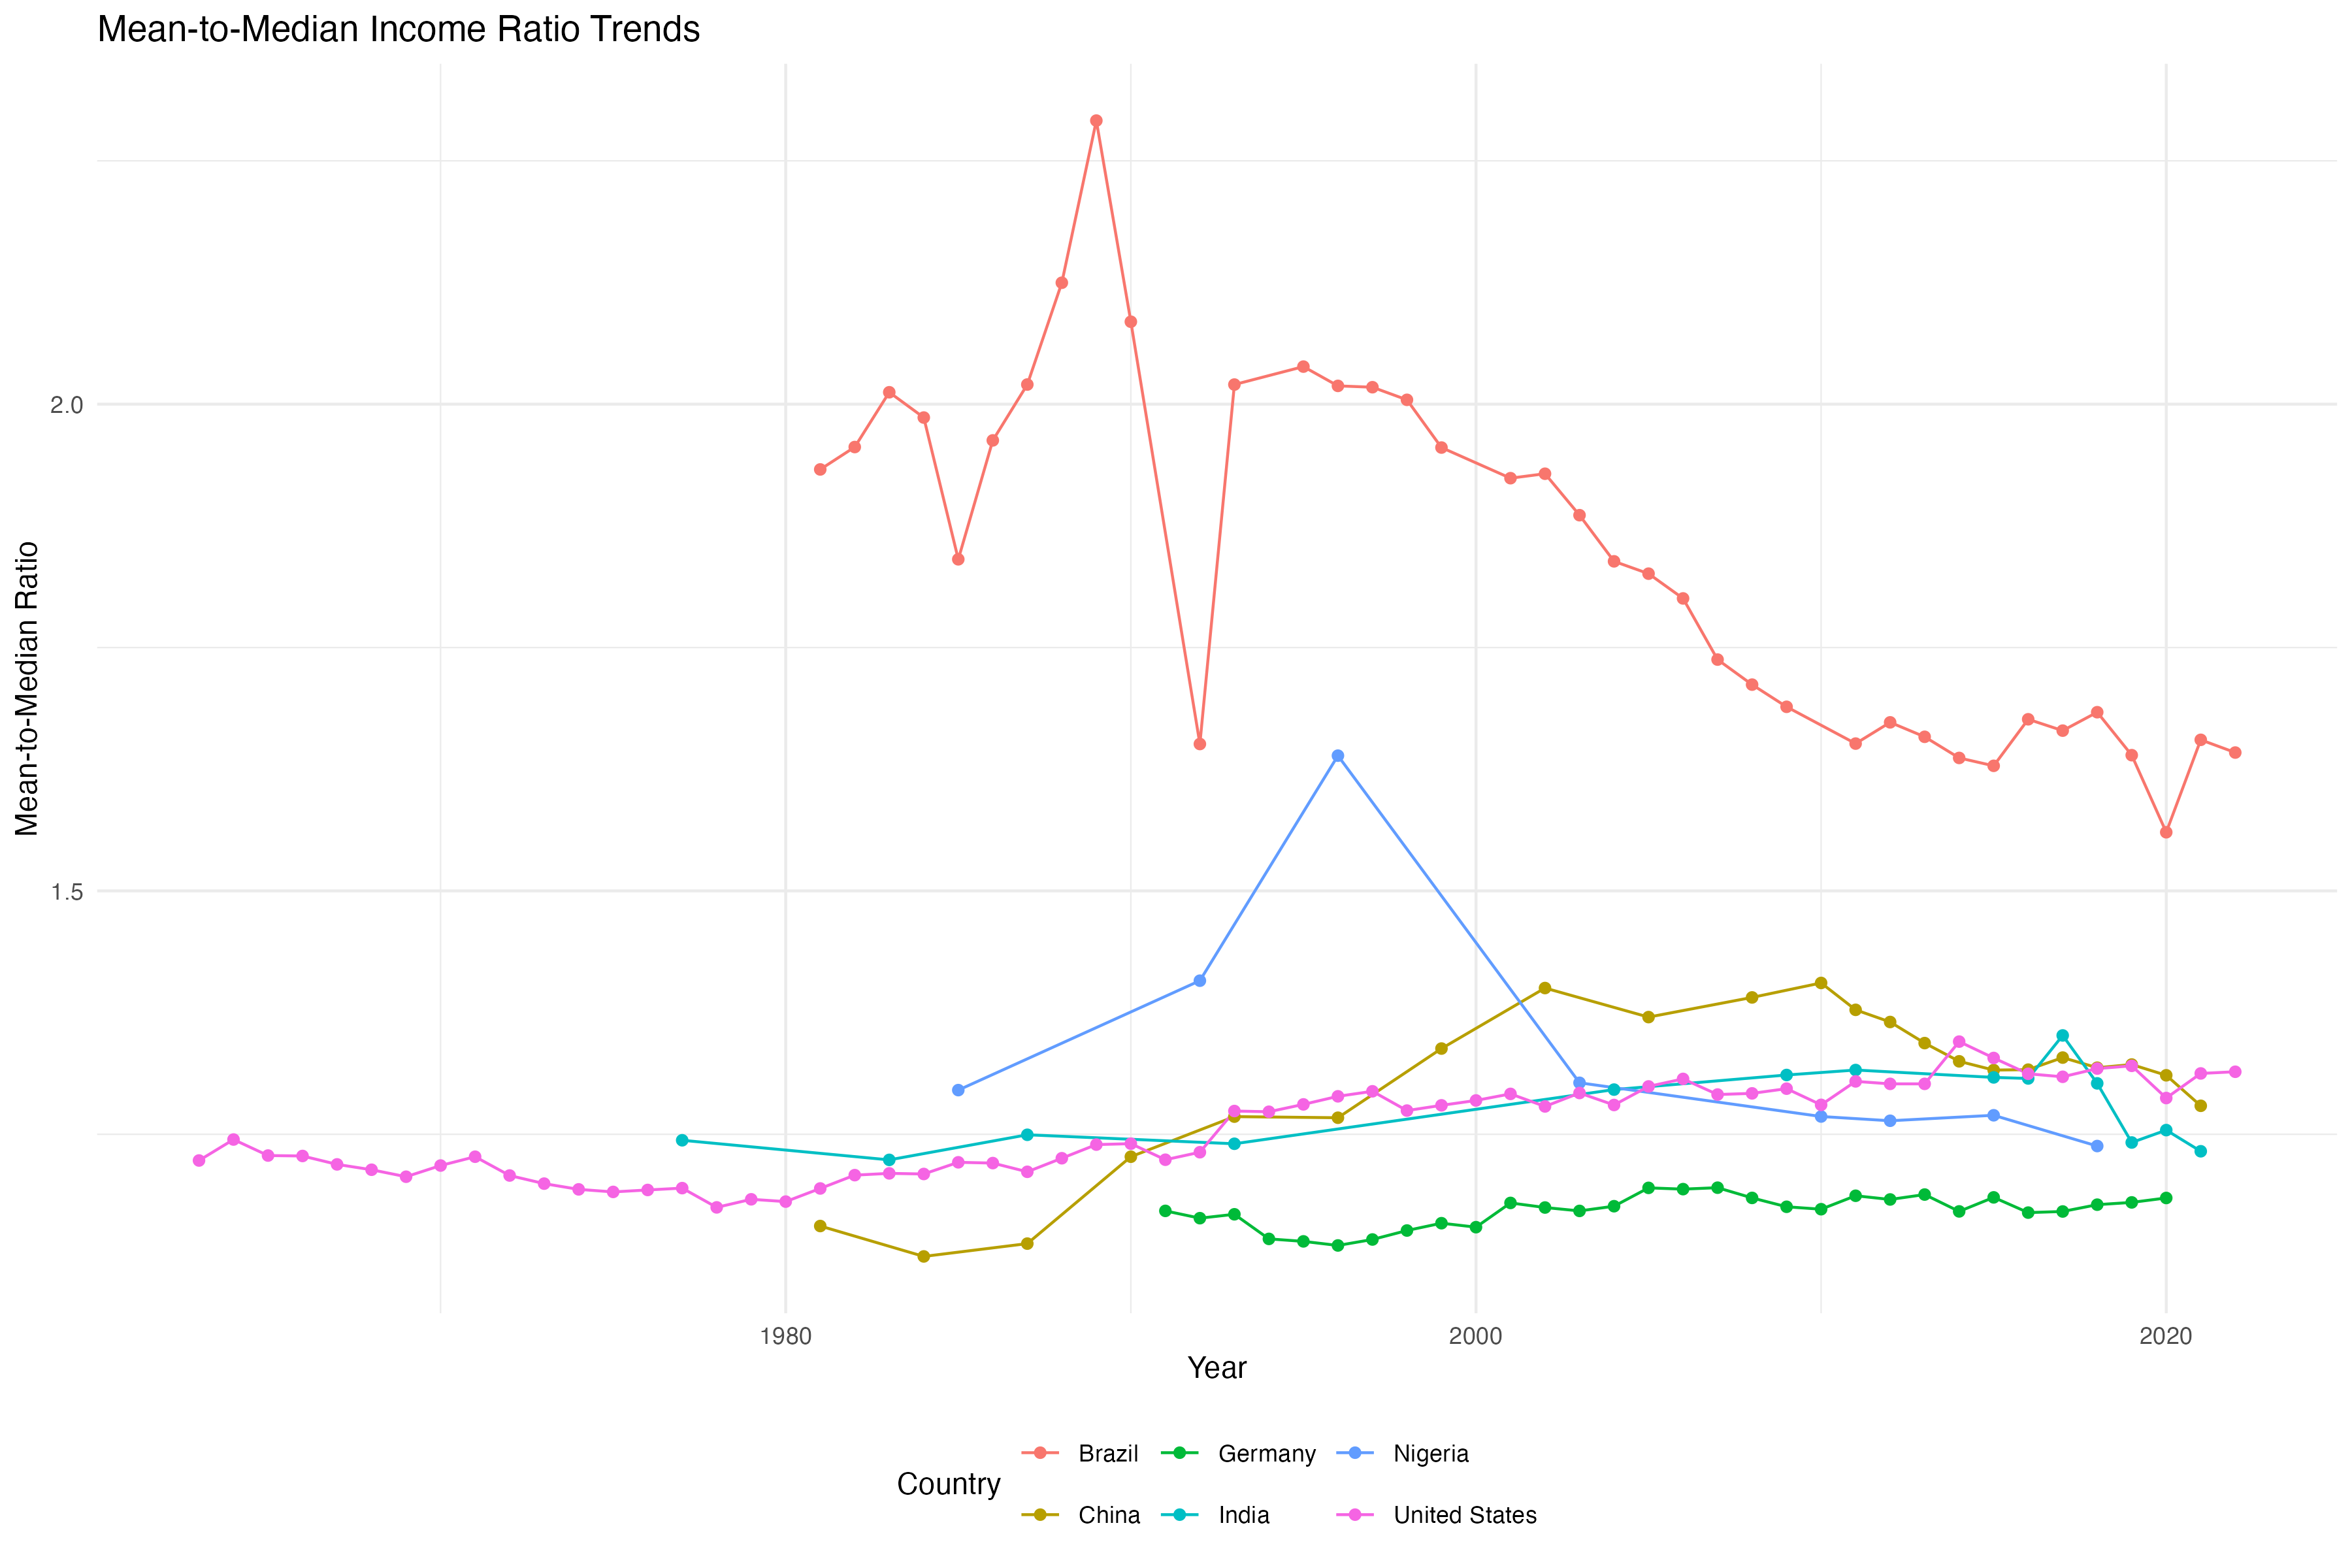
\includegraphics[width=0.8\textwidth]{../output/visualizations/country_mean_median_trends.png}
\caption{Country-Specific Mean-to-Median Ratio Trends}
\end{figure}

\begin{figure}[h]
\centering
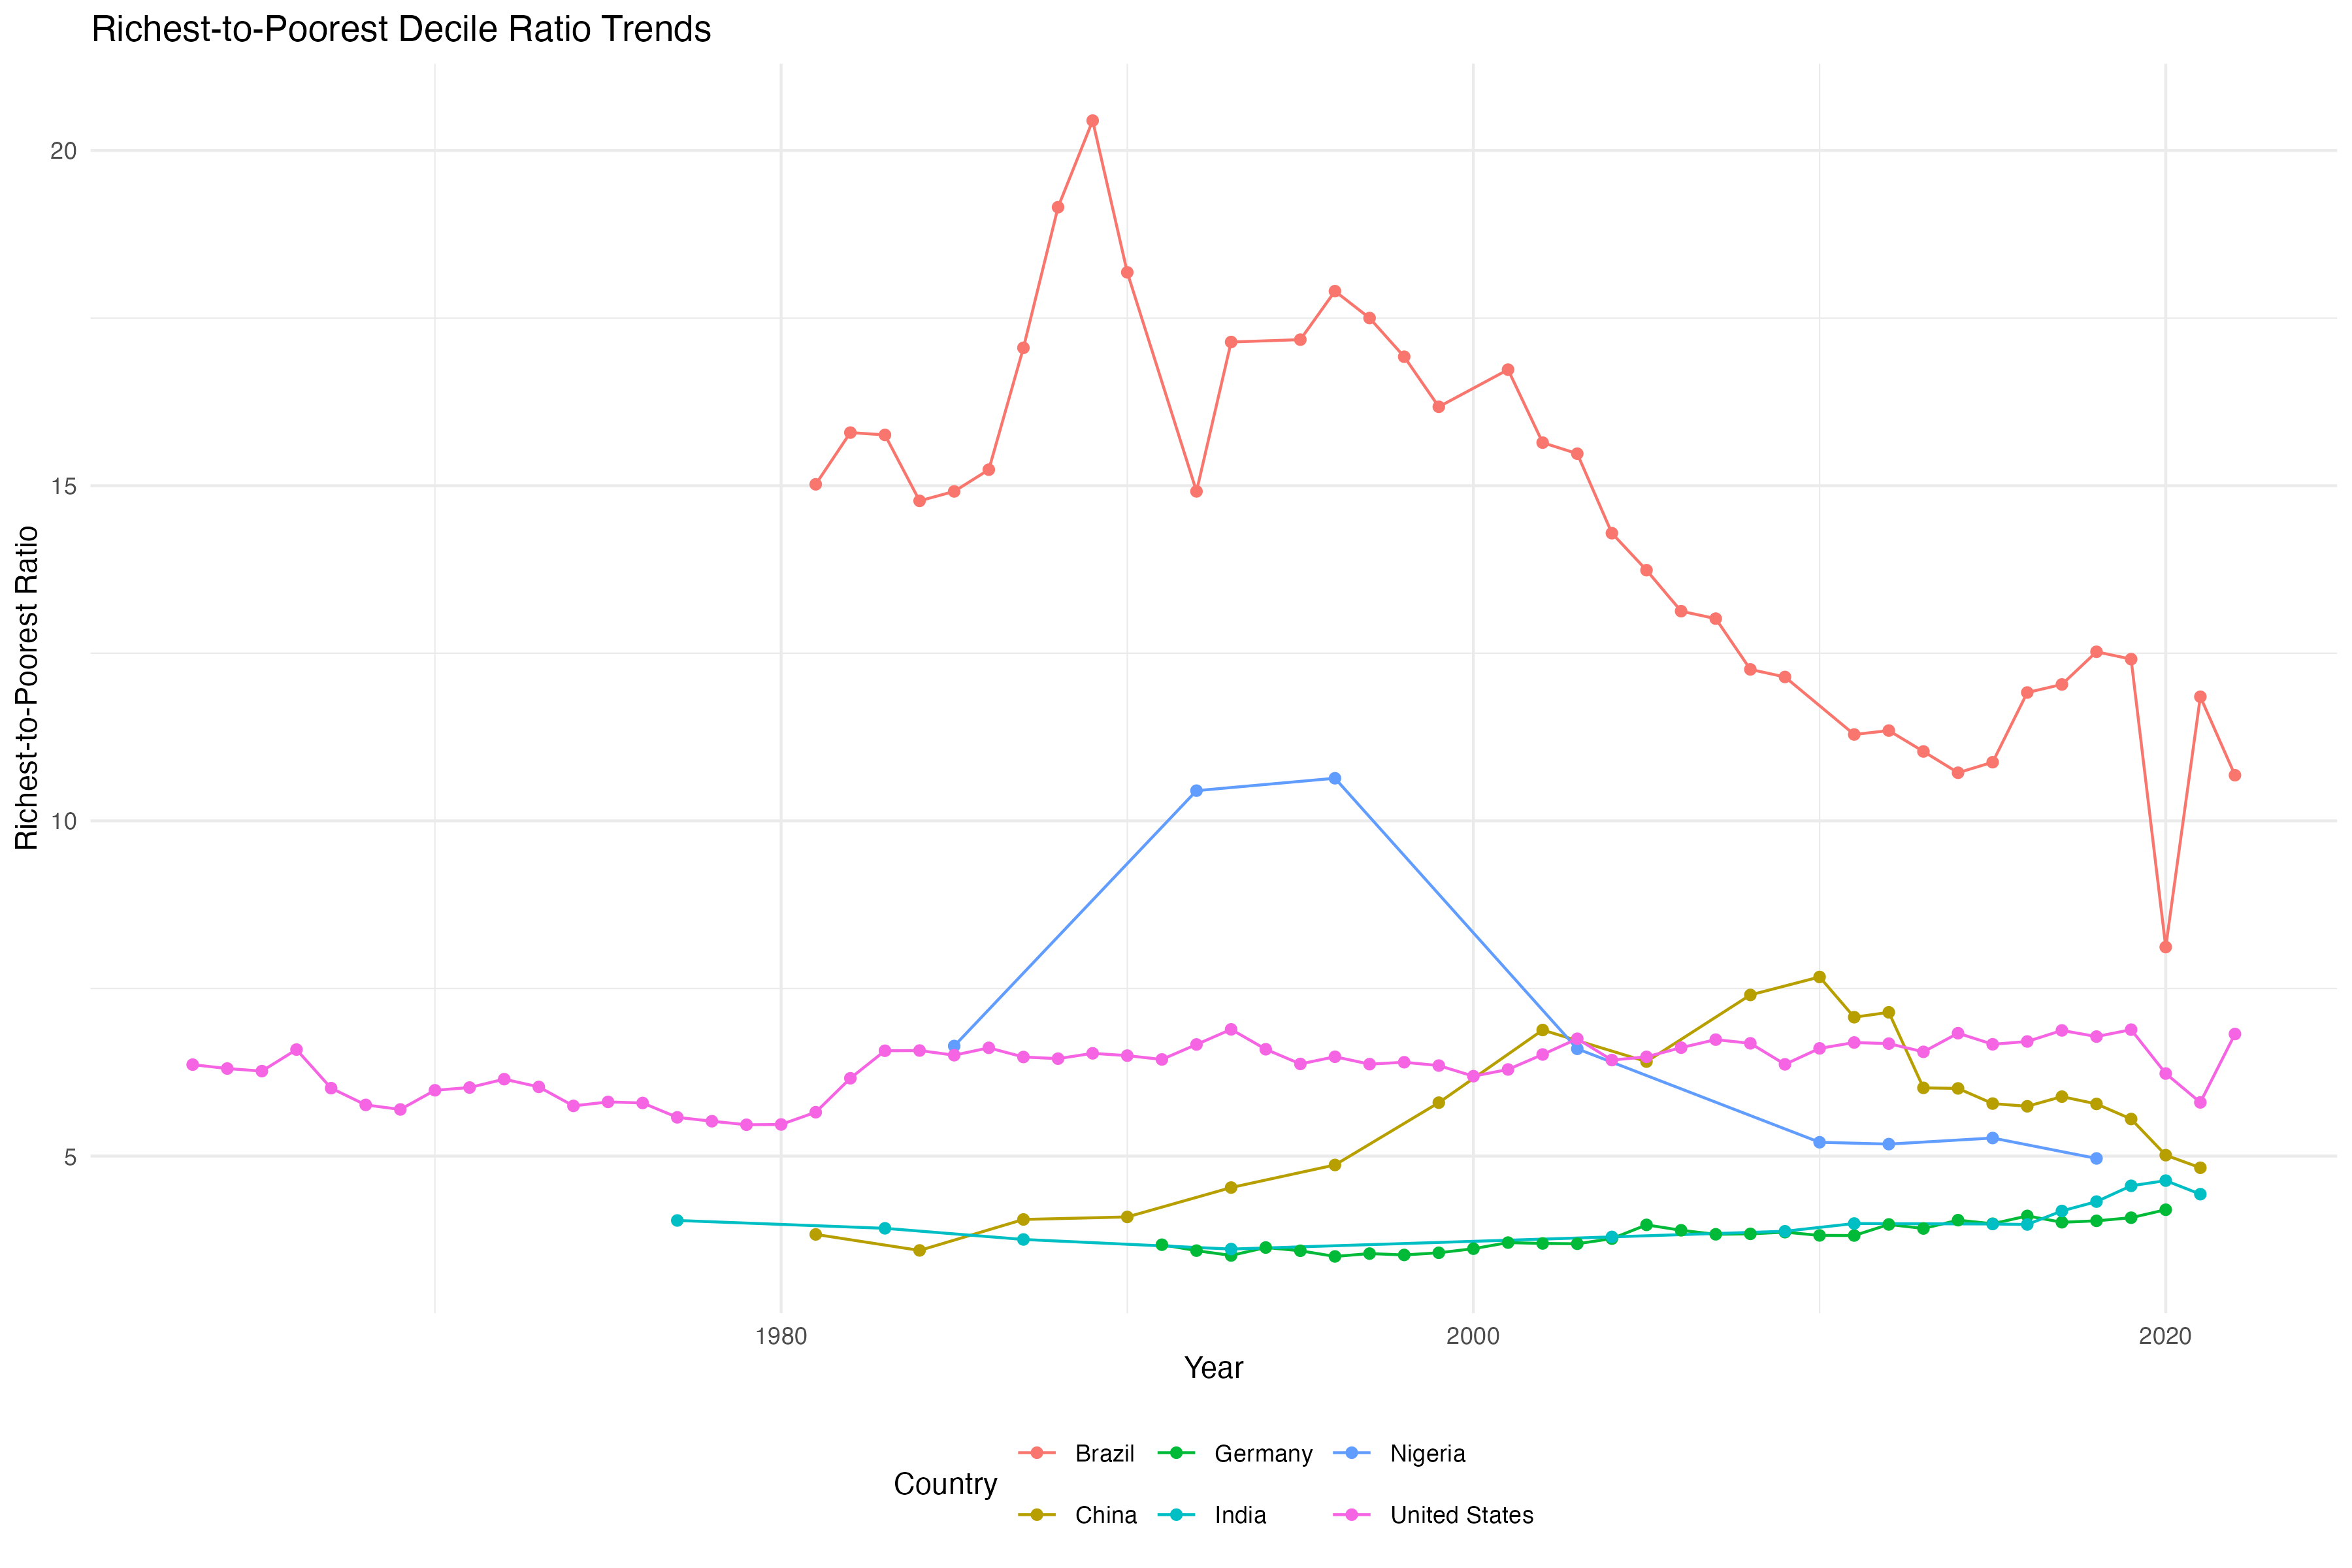
\includegraphics[width=0.8\textwidth]{../output/visualizations/country_rich_poor_trends.png}
\caption{Country-Specific Richest-to-Poorest Ratio Trends}
\end{figure}

\subsection{Regional Analysis}
Our ANOVA analysis indicated significant differences in poverty rates between regions (F = 33.27, p < 0.001), supporting our third hypothesis (H3). The ANOVA F-statistic of 33.27 indicates that regional differences explain a significant portion of the variance in poverty rates. The model's R$^2$ of 0.064 indicates that regional differences alone account for approximately 6.4\% of the variance in poverty rates globally.

Tukey's HSD test revealed five significant pairwise differences between regions. East Asia had significantly lower poverty rates than other regions by the end of the study period, while Latin America had significantly higher rates than Europe. The greatest regional difference was between Europe and East Asia (difference = -14.05 percentage points, p < 0.001), while the smallest significant difference was between Other regions and Europe (difference = 3.46 percentage points, p < 0.001).

The regional trends analysis showed that East Asia experienced the most dramatic reduction in poverty rates, from around 90\% in the early 1980s to near zero by 2020. Latin America showed moderate progress, while Europe maintained consistently low poverty rates throughout the period.

Regional inequality trends revealed distinctive patterns across regions. Latin America consistently had the highest inequality levels (richest-to-poorest ratio around 15-20 and Gini coefficients averaging 0.52), though with a declining trend. East Asia maintained moderate inequality levels (average Gini of 0.39) throughout its rapid poverty reduction period. Europe showed the lowest and most stable inequality measures (Gini coefficients averaging 0.31). These findings suggest that while some minimum level of inequality may be unavoidable or even necessary for economic dynamism, excessive inequality appears to impede poverty reduction efforts.

These regional patterns highlight how different development paths can lead to varying outcomes in terms of poverty reduction. East Asia's approach of combining strong economic growth with moderate levels of inequality appears to have been particularly effective at reducing extreme poverty.

\begin{figure}[h]
\centering
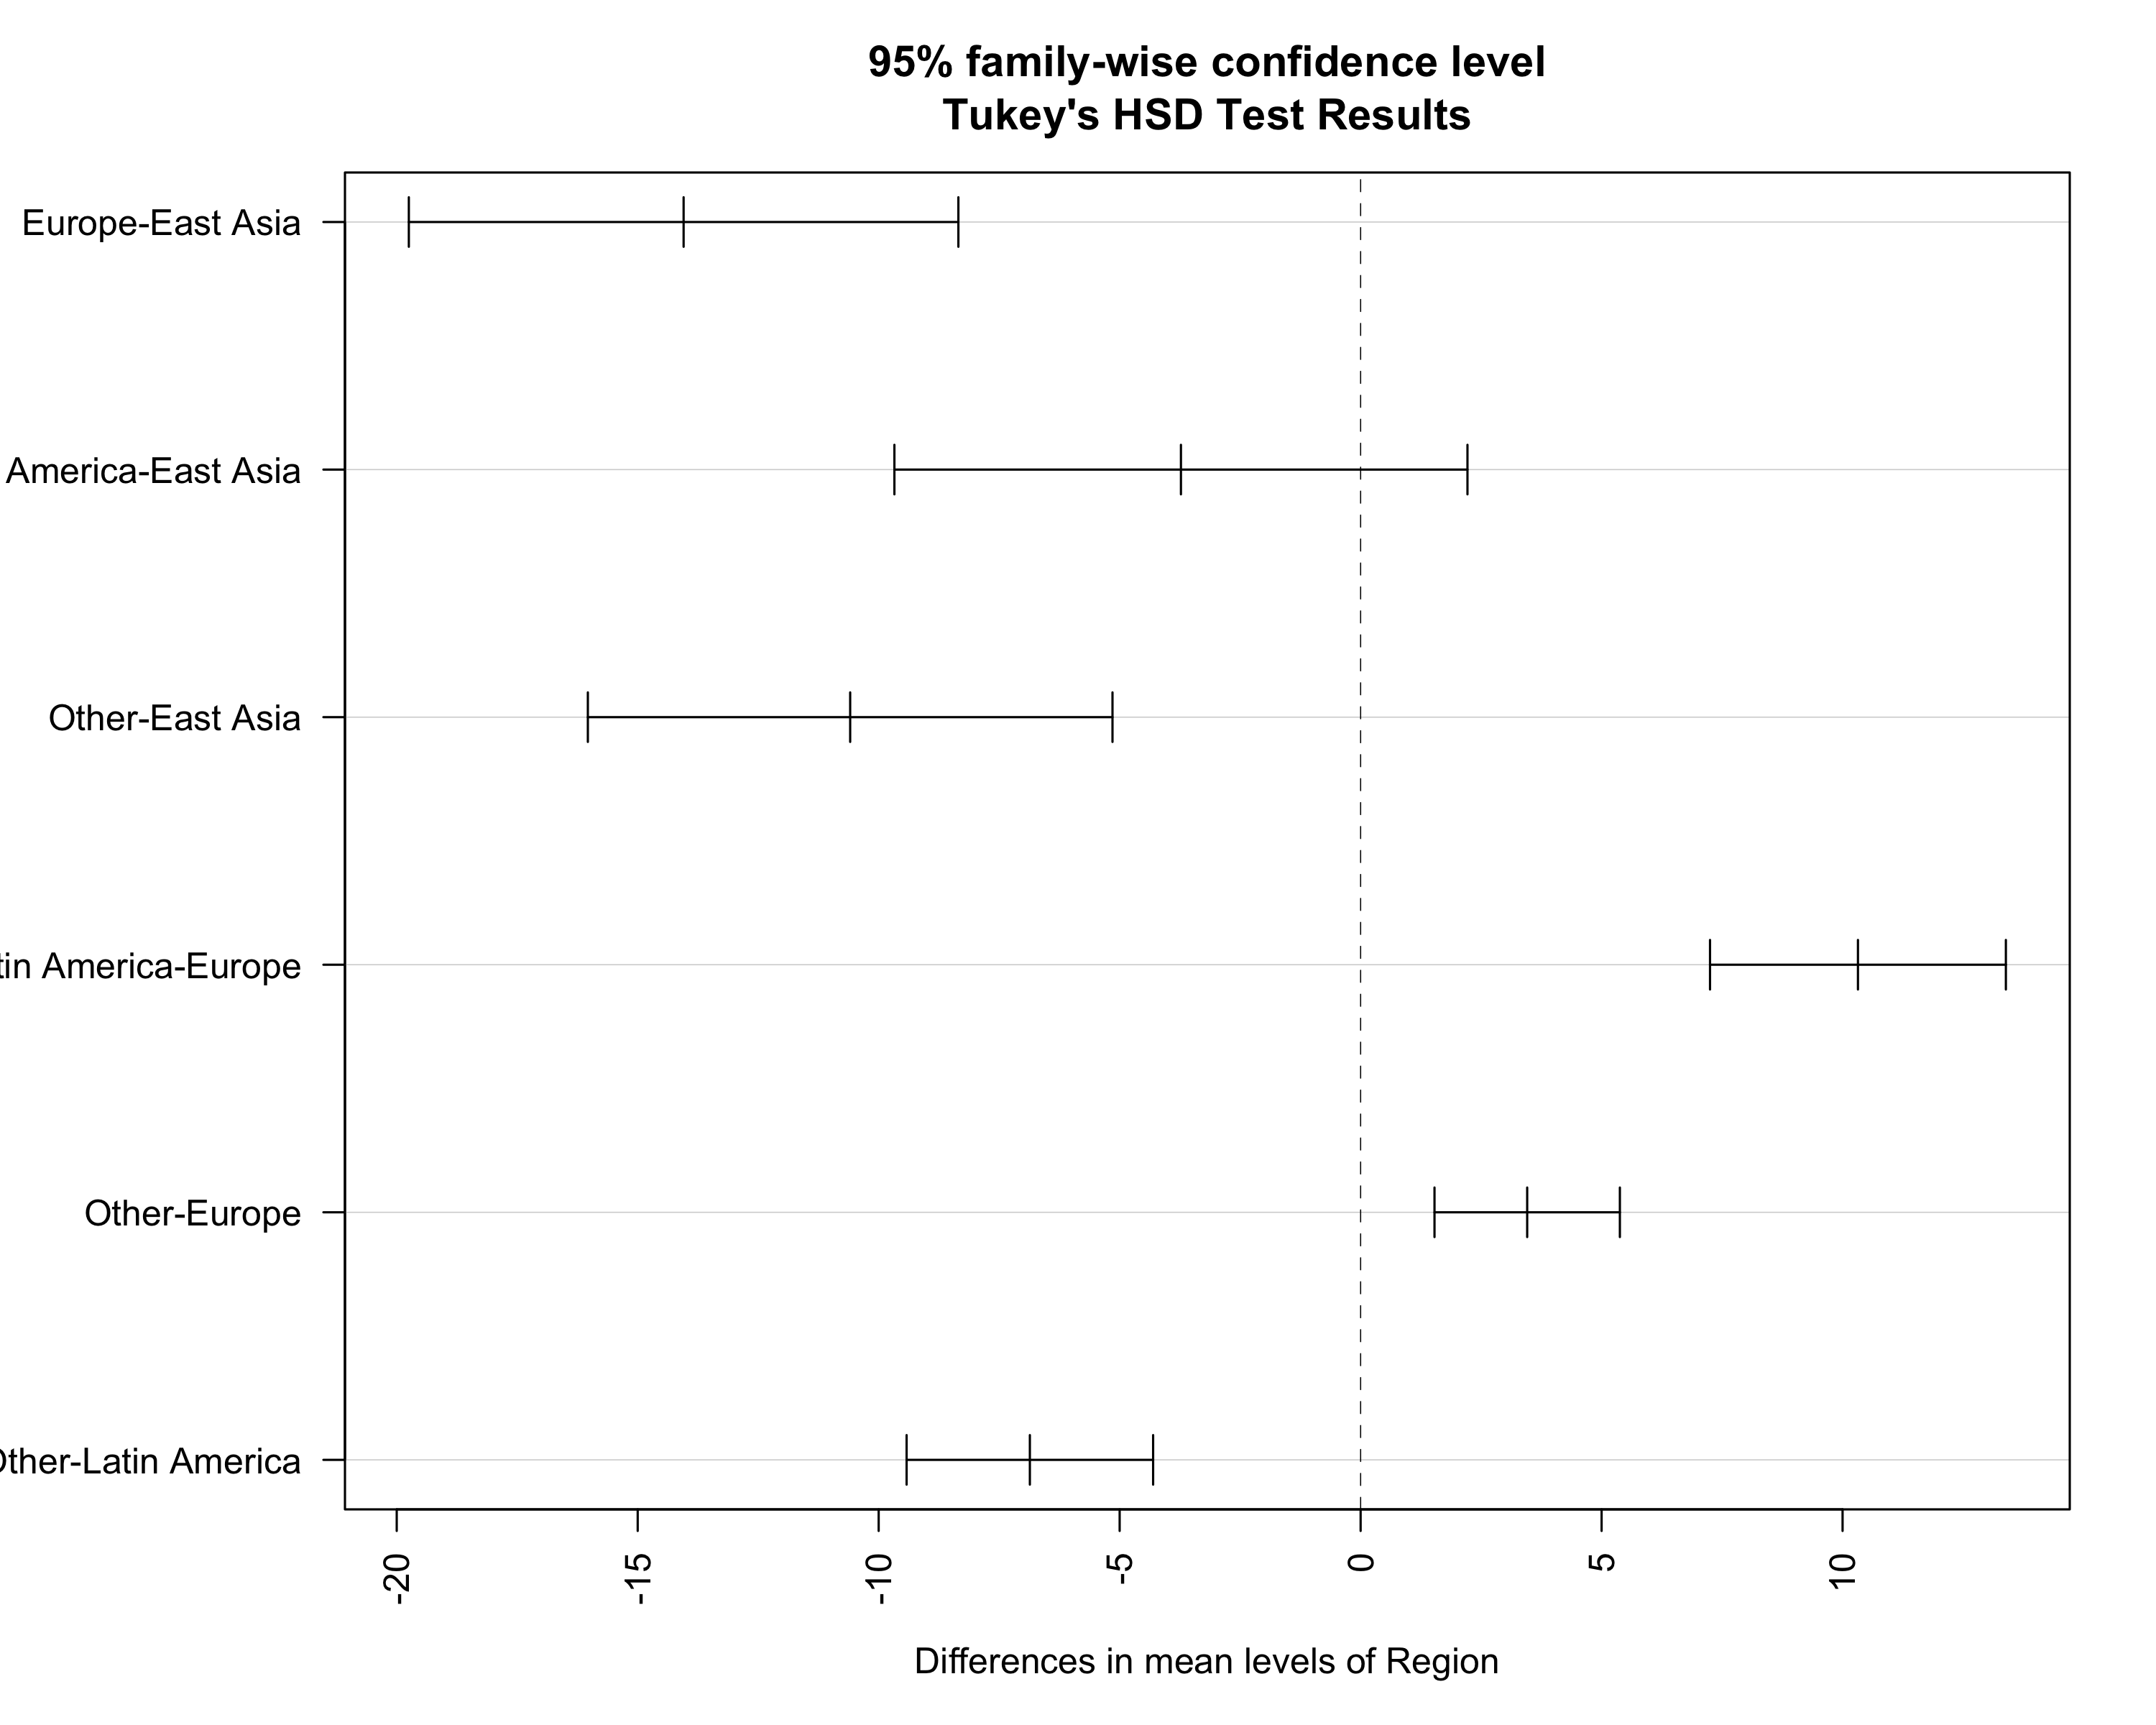
\includegraphics[width=0.8\textwidth]{../output/visualizations/tukey_hsd_results.png}
\caption{Tukey's HSD Test Results for Regional Comparisons}
\end{figure}

\subsection{Regression Analysis}
Our regression analysis provided deeper insights into the relationship between income, inequality, and poverty:

Our progression of models reveals the incremental explanatory power of including additional variables:
\begin{enumerate}
    \item \textbf{Model 1 (Income-Only):} A log-linear model of extreme poverty on mean income explained 24.8\% of the variance in poverty rates (R$^2$ = 0.248). 
    \begin{itemize}
        \item F-statistic: 484.6 on 1 and 1460 DF, p < 2.2e-16
        \item The coefficient on log(Mean\_Income) was -9.57 (p < 0.001), indicating that a 10\% increase in mean income is associated with a 0.957 percentage point decrease in extreme poverty.
    \end{itemize}
    \item \textbf{Model 2 (Inequality-Only):} A linear model of extreme poverty on the richest-to-poorest ratio explained 17.9\% of the variance (R$^2$ = 0.179). 
    \begin{itemize}
        \item F-statistic: 322.1 on 1 and 1460 DF, p < 2.2e-16
        \item The coefficient on Richest\_to\_Poorest\_Ratio was 0.43 (p < 0.001), indicating that a one-unit increase in the ratio is associated with a 0.43 percentage point increase in extreme poverty.
    \end{itemize}
    \item \textbf{Model 3 (Combined):} A model including both income and inequality explained 35.2\% of the variance (R$^2$ = 0.352), a 41.9\% improvement over Model 1. 
    \begin{itemize}
        \item Both predictors remain highly significant (p < 0.001)
        \item Income coefficient decreases to -7.21, showing that part of income's effect was actually capturing inequality
    \end{itemize}
    \item \textbf{Model 4 (Interaction):} Our most comprehensive model included an interaction between income and inequality, along with the mean-to-median ratio. This model explained 57.9\% of the variance in poverty rates (R$^2$ = 0.579), a 64.5\% improvement over Model 3. 
    \begin{itemize}
        \item The coefficient for log(Mean\_Income) was -2.88, indicating that a 1\% increase in mean income is associated with a 0.0288 percentage point decrease in poverty, holding other factors constant.
        \item The significant negative interaction term (-0.983, p < 0.001) indicates that the poverty-reducing effect of higher income is stronger in more equal societies.
        \item For a country with a richest-to-poorest ratio of 5, a 10\% increase in mean income reduces poverty by approximately 0.78 percentage points [(-2.875 - 0.983 $\times$ 5) $\times$ 0.1]
        \item For a country with a ratio of 10, the same income increase reduces poverty by only 0.29 percentage points [(-2.875 - 0.983 $\times$ 10) $\times$ 0.1]
        \item This demonstrates numerically how inequality dramatically dampens the poverty-reducing effects of economic growth.
    \end{itemize}
\end{enumerate}

\begin{figure}[h]
\centering
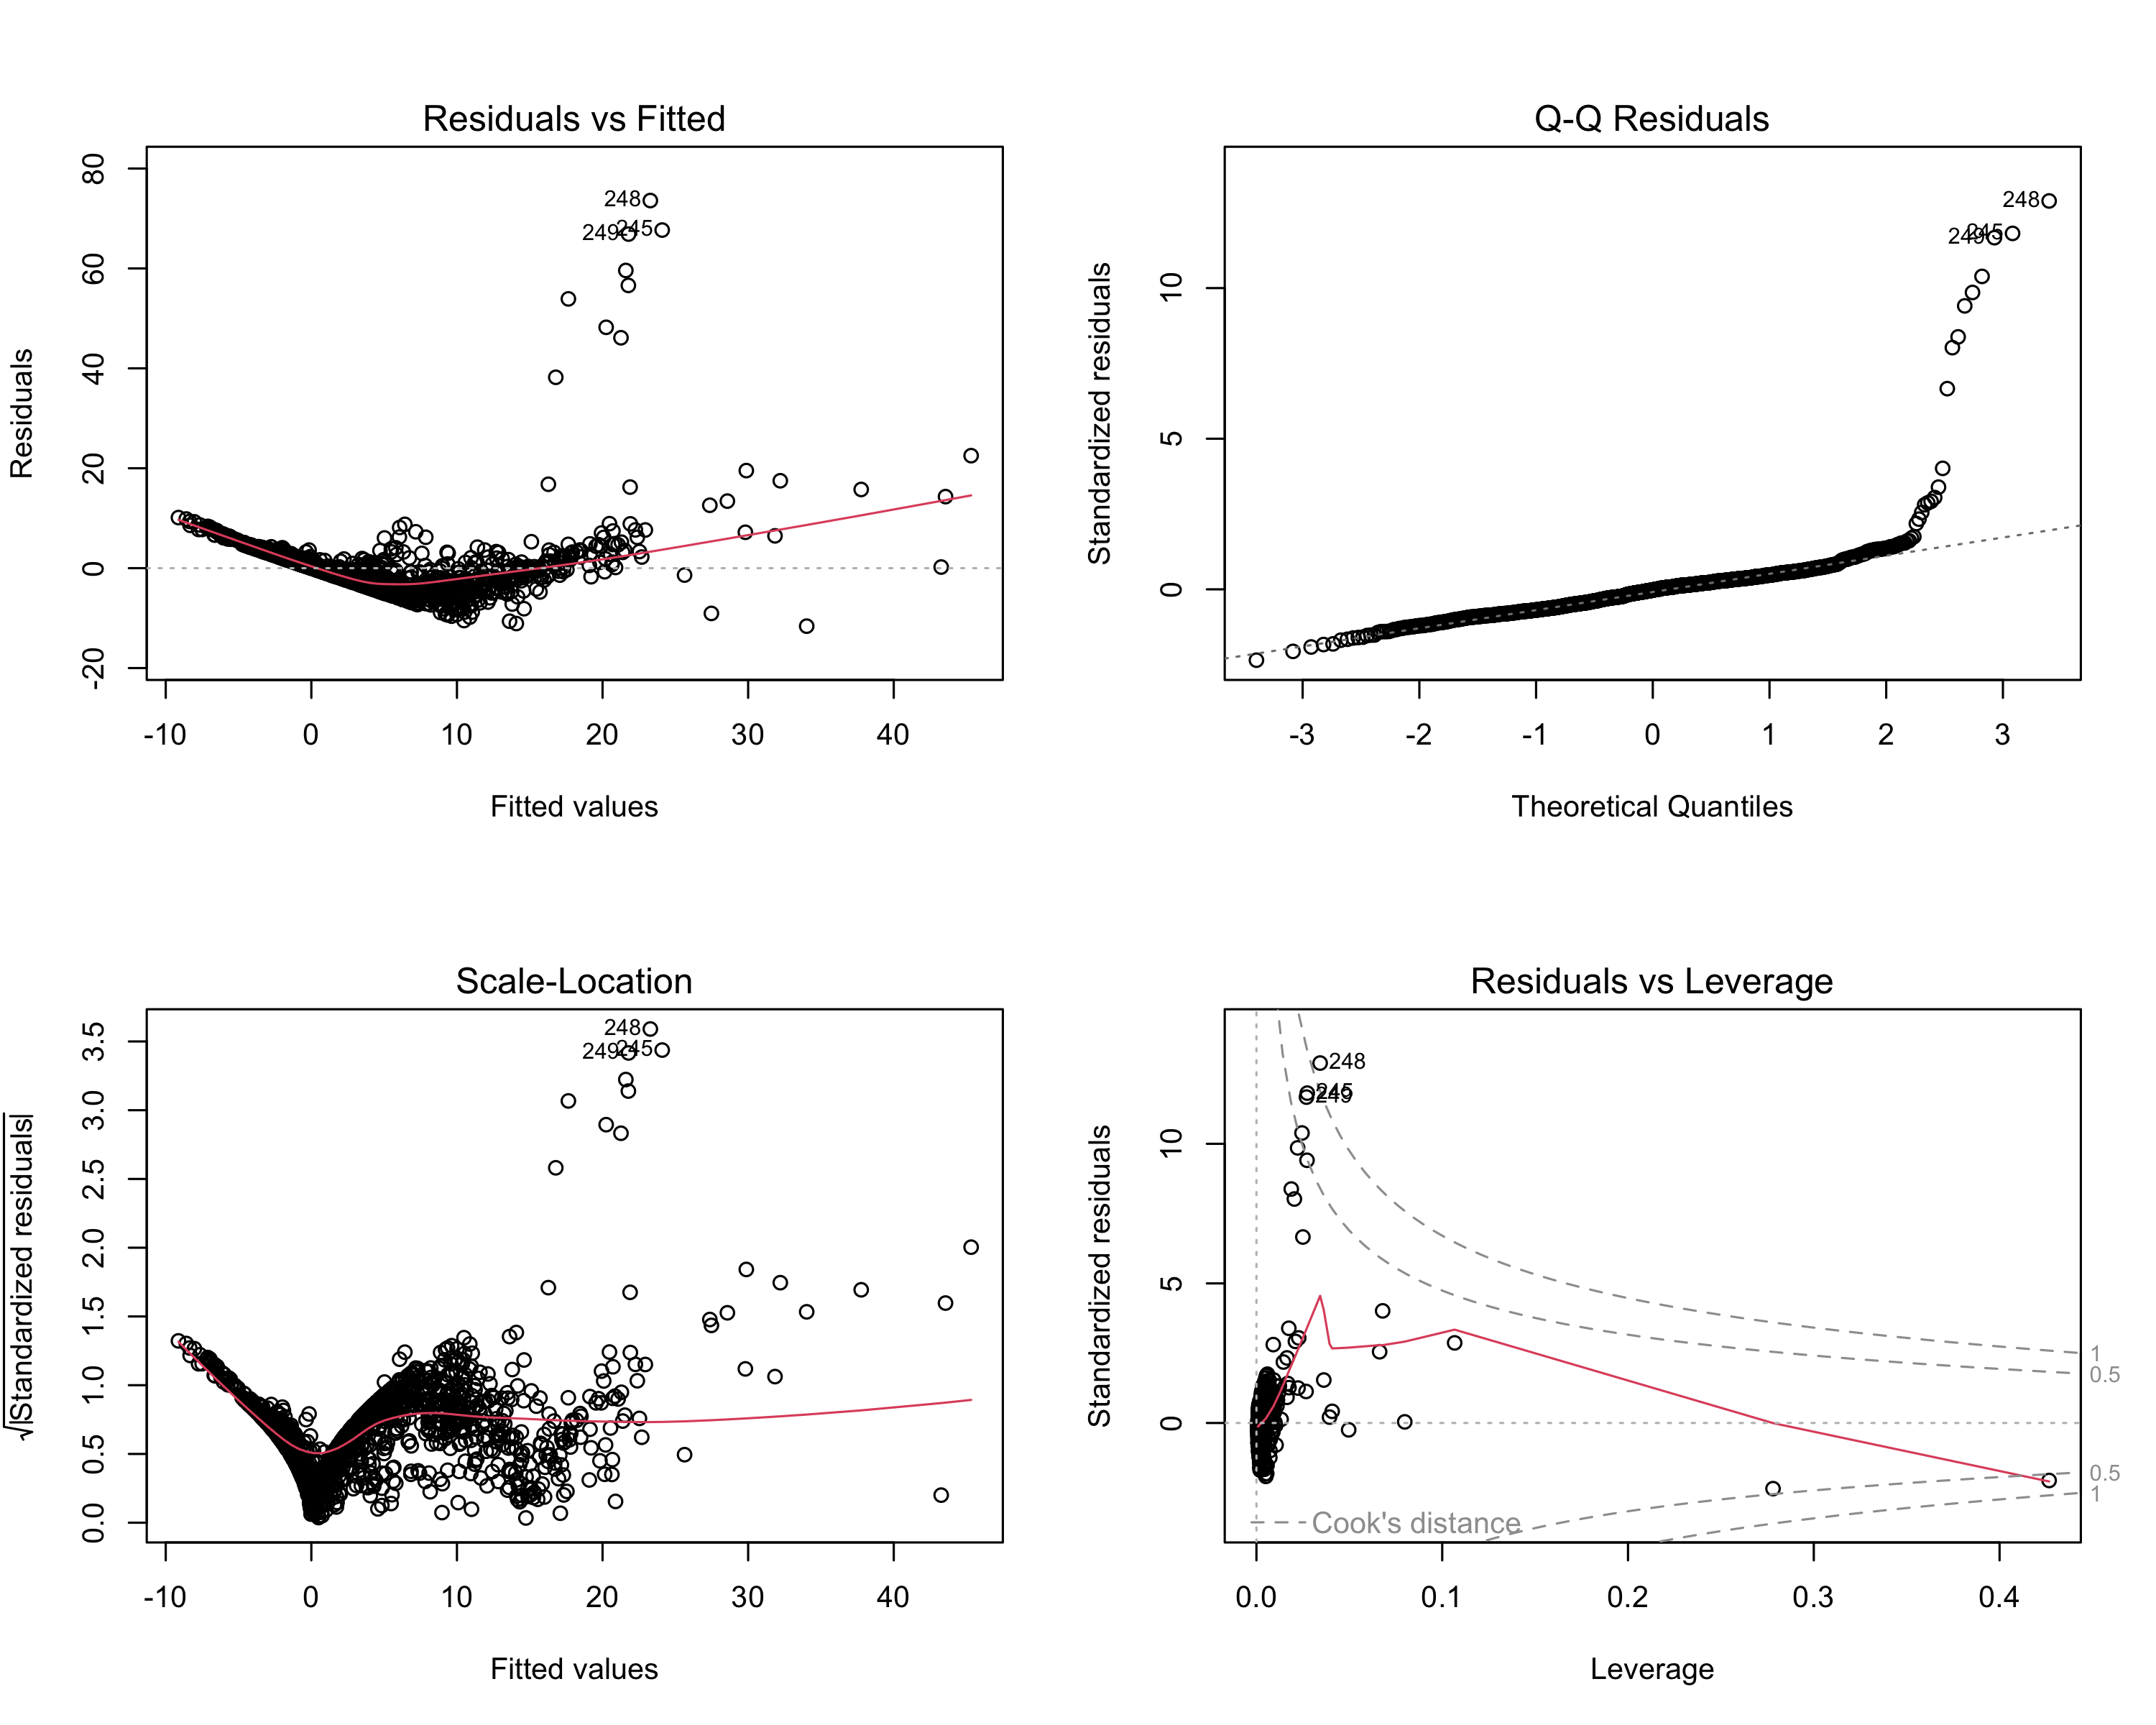
\includegraphics[width=0.8\textwidth]{../output/visualizations/advanced_model_diagnostics.png}
\caption{Advanced Model Diagnostic Plots}
\end{figure}

Diagnostic tests revealed some heteroscedasticity in the residuals, suggesting that the model may be less accurate for countries with very high poverty rates. However, the Durbin-Watson test did not indicate significant autocorrelation in the residuals.

These regression results strongly support our second hypothesis (H2), demonstrating that the relationship between economic growth and poverty reduction is significantly moderated by income distribution patterns.

\subsection{Poverty Reduction Success Analysis}
We identified countries with at least 5 data points spanning 10+ years and calculated their poverty reduction metrics. The most successful countries in reducing extreme poverty (measured by relative reduction) were:
\begin{enumerate}
    \item Malaysia: 100\% reduction (from 2.68\% to 0\%)
    \item South Korea: 100\% reduction (from 0.25\% to 0\%)
    \item Chile: 97.4\% reduction (from 15.4\% to 0.40\%)
    \item Costa Rica: 96.6\% reduction (from 25.9\% to 0.88\%)
    \item Lithuania: 96.2\% reduction (from 6.62\% to 0.25\%)
\end{enumerate}

When examining the characteristics of successful countries, we found they typically combined strong economic growth with stable or decreasing inequality. For example, Chile's richest-to-poorest ratio decreased from 11.2 to 9.6 while its mean income increased from \$12.3 to \$29.7 during the period of substantial poverty reduction.

This analysis provides partial support for our fourth hypothesis (H4), as countries with more balanced growth across income segments (including the poorest decile) achieved more substantial poverty reductions.

\subsection{Time Series Analysis and Forecasting}
Our time series analysis used an ARIMA(1,0,2) model with non-zero mean for forecasting global poverty rates. The model parameters were:
\begin{itemize}
    \item AR(1): 0.7088
    \item MA(1): -0.9113
    \item MA(2): 0.8056
    \item Mean: 3.9242
\end{itemize}

Our ARIMA(1,0,2) model with coefficients AR(1) = 0.7088, MA(1) = -0.9113, MA(2) = 0.8056, and mean = 3.9242 yielded a forecast with 95\% confidence intervals ranging from -1.73 to 9.83 for poverty rates five years ahead. This wide interval (spanning 11.56 percentage points) reflects considerable uncertainty in future poverty trends.

The model's MAPE (Mean Absolute Percentage Error) of 94.49\% indicates challenges in fitting the historical volatility in poverty rates, particularly around spike periods in the 1980s and early 1990s.

The time series decomposition revealed that the global poverty trend showed a non-linear pattern, with a peak in the early 1980s followed by a decline that has slowed in recent years. The moving average trend component captured the major movements in poverty rates, while the random component showed no clear cyclical pattern.

Our trend analysis compared linear and polynomial models, with the polynomial model providing a much better fit (AIC = 355.08 vs. 373.05). This confirms that global poverty reduction has not followed a steady pace but has experienced periods of acceleration and deceleration over the study period.

\section{Conclusion and Implications}\label{sec:conclusion}
Our comprehensive analysis of global income distribution and poverty dynamics has yielded several important findings with implications for development policies and strategies:
\begin{enumerate}
    \item \textbf{Income-Inequality-Poverty Nexus:} Our results confirm a complex relationship between income, inequality, and poverty. While higher income levels are generally associated with lower poverty rates, the strength of this relationship depends on income distribution. The significant interaction between income and inequality in our regression model indicates that economic growth is more effective at reducing poverty in more equal societies.
    \item \textbf{Global Progress and Challenges:} We observe a general trend of decreasing global poverty and a modest reduction in global inequality over the study period. However, progress has been uneven across regions and countries, with East Asia showing the most dramatic improvements while other regions have seen slower progress.
    \item \textbf{Regional Disparities:} The significant differences in poverty rates and trends between regions highlight the importance of tailored development strategies that address region-specific challenges. East Asia's success suggests that combining economic growth with moderate levels of inequality can lead to substantial poverty reduction.
    \item \textbf{Success Factors:} Countries that have been most successful at reducing extreme poverty typically combined strong economic growth with stable or decreasing inequality. The experiences of countries like Malaysia, Chile, and Costa Rica demonstrate that reducing inequality can enhance the poverty-reducing impact of economic growth.
    \item \textbf{Methodological Insights:} Our analysis shows that multiple metrics of inequality (mean-to-median ratio, richest-to-poorest ratio, and Gini coefficient) provide complementary insights into income distribution. The Gini coefficient showed the strongest correlation with poverty rates (r = 0.531), followed by the mean-to-median ratio (r = 0.508), suggesting that these standard measures of income distribution skewness may be particularly important factors in understanding poverty dynamics.
\end{enumerate}

\subsection{Research Questions Revisited}
Our analysis addressed each of our initial research questions:
\begin{enumerate}
    \item \textbf{How does income distribution shape the relationship between economic growth and poverty reduction?} Our findings confirm that income distribution significantly moderates the relationship between economic growth and poverty reduction. The significant interaction between income and inequality in our Model 4 ($\beta$ = -0.983, p < 0.001) demonstrates that economic growth is more effective at reducing poverty in more equal societies.
    \item \textbf{How do different measures of inequality correlate with poverty reduction rates?} We found that both inequality metrics (mean-to-median ratio and richest-to-poorest ratio) were positively correlated with poverty rates (r = 0.508 and r = 0.428, respectively). The mean-to-median ratio showed a stronger correlation, suggesting that income distribution skewness may be particularly important for understanding poverty dynamics.
    \item \textbf{Which countries have successfully reduced both poverty and inequality?} Our analysis identified several success stories, particularly Malaysia, South Korea, Chile, Costa Rica, and Lithuania, which achieved relative poverty reductions of over 96\%. These countries typically combined strong economic growth with stable or decreasing inequality.
    \item \textbf{How do growth rates of different income segments relate to overall poverty reduction?} Our analysis of country-specific patterns showed that countries with more balanced growth across income segments achieved more substantial poverty reductions. This was particularly evident in East Asia, where growth benefited both the poorest and richest segments, leading to the most dramatic poverty reduction among all regions.
\end{enumerate}

\subsection{Limitations and Future Research}
Our study has several limitations that suggest directions for future research:
\begin{enumerate}
    \item \textbf{Data Coverage:} Despite our comprehensive datasets, there are gaps in coverage for certain countries and time periods, particularly for low-income countries where poverty is most prevalent.
    \item \textbf{Causality:} Our analysis identifies correlations but cannot definitively establish causal relationships between income distribution and poverty reduction. Future research could employ instrumental variable approaches or natural experiments to address potential endogeneity.
    \item \textbf{Policy Mechanisms:} More research is needed to identify the specific policy mechanisms through which countries have achieved both economic growth and equitable distribution. Case studies of successful countries could provide valuable insights into effective policy approaches.
    \item \textbf{Multidimensional Poverty:} Our focus on income-based poverty measures does not capture other dimensions of poverty such as access to education, healthcare, and basic services. Future research could incorporate multidimensional poverty measures to provide a more holistic view of poverty reduction.
\end{enumerate}

In conclusion, our findings suggest that development strategies focusing solely on economic growth without addressing distributional concerns may be less effective at reducing poverty. Policies that promote both growth and equity are likely to be most successful at improving the lives of the poorest citizens and achieving the global goal of eliminating extreme poverty.

\clearpage
\section{References}
\bibliographystyle{plain}
\bibliography{references}
\end{document}